\documentclass[a4paper,11pt]{article}
\author{ 杨旭鹏  \  PB17000234}
\date{2019年秋季}
\title{计算物理A 第十三题}

\usepackage{ctex}
\usepackage{amsmath}
\usepackage{amsfonts}
\usepackage{graphicx}
\usepackage{epstopdf}
\usepackage{lastpage}
\usepackage{hyperref}
\usepackage{listings}
\RequirePackage{xcolor}
\usepackage{appendix}
\usepackage{caption2}
\usepackage{subfigure}
\usepackage{float}
\usepackage{verbatim}
\usepackage{fancybox}
\makeatletter\def\@captype{table}\makeatother

\definecolor{dkgreen}{rgb}{0,0.6,0}
\definecolor{gray}{rgb}{0.5,0.5,0.5}
\definecolor{mauve}{rgb}{0.58,0,0.82}

\lstset{
  frame=tb,
  aboveskip=3mm,
  belowskip=3mm,
  showstringspaces=false,
  columns=flexible,
  framerule=1pt,
  rulecolor=\color{gray!35},
  backgroundcolor=\color{gray!5},
  basicstyle={\small\ttfamily},
  numbers=left,
  numberstyle=\tiny\color{gray},
  keywordstyle=\color{blue},
  commentstyle=\color{dkgreen},
  stringstyle=\color{mauve},
  breaklines=true,
  breakatwhitespace=true,
  tabsize=3,            
  }



\begin{document}
\maketitle
\tableofcontents

\section{题目描述}
进行单中心DLA模型的模拟(可以用圆形边界,也可以用正方形边界),并 用两种方法计算模拟得到的DLA图形的分形维数,求分形维数时需要作出双对数图。 
\section{算法}
将二维平面划分为一个个正方形格点,点阵中⼼放置⼀个种⼦粒⼦作为凝聚中⼼,在距离种⼦某距离的产生边界上随机产⽣⼀个粒⼦,使其做随机⾏⾛。当粒⼦⾛到与团簇粒子相接触时,就被粘住不动,成为团簇的⼀部分;当粒⼦越过远离中⼼某距离的逃离边界时,粒⼦被判定逃离,重新由起始位置开始随机行走。当团簇不断扩大时,产生边界和逃离边界跟随变大。直到团簇的大小为规定值时,停止。

此程序利用二维数组表示二维平面上的格点,原点处于二维数组的中心位置。规定二维数组的边界距离中心有$LEN$个单位长度(即二维数组的形状为$(2LEN+1)\times (2LEN+1)$,原点的行号和列号均为$LEN$)。规定粒子随机行走一步只能向上,向下,向左或向右移动一个单位长度(即一格)且朝四个方向移动的概率相同。当粒子周围8个格点有团簇粒子时,判定该粒子粘连到团簇粒子,停止随机行走,将此位置所对应的二维数组的值改为1,表示此处有粒子,并在产生边界上随机产生一新的粒子,重复此过程。



\subsection{程序子函数介绍}
\subsubsection{随机粒子初始位置产生器}
传入参数包括一在$(0,1)$均匀抽取的随机值(由16807产生器产生)和产生边界距离原点的大小$r$。例如对于圆形边界,将传入进来的随机值$\times 2\pi $即得到在$(0,2\pi)$均匀抽取的随机值$\theta$作为粒子起始位置在极坐标系下的角度值。则随机粒子初始位置的$(x,y)$坐标分别为$round(r cos(\theta))$和$round(r sin(\theta))$。其中$round()$为四舍五入函数,因为最后初始位置要落实到某个格点上。则随机粒子在二维矩阵上的行号$i$和列号$j$分别为$x+LEN$和$y+LEN$。


\subsubsection{粒子随机行走器}
传入参数为粒子的初始位置;逃逸边界半径;二维平面对应的二维矩阵;在$[-2^{31},2^{31}-1]$均匀抽取的随机整数,用于作为产生随机数的种子。利用16807产生器产生均匀分布在$[0,1]$的随机数,对于此粒子的第$k$步来说,若第$k$个随机数$\in (0,\frac{1}{4}]$,则向x轴正方向走一个单位长度;若$\in (\frac{1}{4},\frac{1}{2}]$,向x轴负向走一个单位;若$\in (\frac{1}{2},\frac{3}{4}]$,向y轴正向走一个单位;若$\in (\frac{3}{4},1]$,向y轴负向走一个单位。每步结束后,都判断周围8个格点是否有团簇粒子,是否走出逃逸边界。


\subsubsection{盒计数法统计器}
此子程序包含于另一用于数据处理的C程序。将生成好的包含团簇粒子位置信息的二维矩阵传入,程序会统计出以原点为中心,长度为1024个格点的$N(\epsilon)$


\subsubsection{Sandbox统计器}
此子程序包含于另一用于数据处理的C程序。将生成好的包含团簇粒子位置信息的二维矩阵传入,程序会统计出以原点为中心,长度为$11,21,31,\cdots ,601$个格点的$N(r)$



\subsection{16807产生器}
作用中所产生的随机数使用16807产生器产生。16807产生器属于线性同余法产生器的特例。而线性同余法方法为:

\begin{equation}
\begin{aligned}
	I_{n+1} &= (aI_{n} + b) \ mod \ m \\
	x_{n} &= I_{n}/m
\end{aligned}
\label{linear}	
\end{equation}

其中整数$I_{i} \in [0,m-1]$,$a,b,m$为算法中的可调参数,其选取直接影响产生器的质量。选取参数:
\begin{equation}
\left\{
\begin{array}{l}
	a = 7^{5} = 16807 \\
	b = 0 \\
	m = 2^{31}-1 = 2147483647
\end{array}
\right.
\end{equation}

即为所谓的16807产生器。由于直接利用\ref{linear}编写程序时计算$(aI_{n} \ mod \ m )$时很容易造成数据溢出,故采取Schrage方法进行具体编程的实现:

\begin{equation}
aI_{n} \ mod \ m = \left\{
\begin{array}{l}
	a(I_{n}\ mod \ q) - r[I_{n}/q],\ \ \ \ \ \ \ \ if \geq 0 \\
	a(I_{n}\ mod \ q) - r[I_{n}/q] + m,\ \ otherwise	
\end{array}
\right.
\end{equation}

其中$m=aq+r$,即$q=m/a=127773$,$r=m \ mod \ a=2836$。即可利用此方法产生伪随机数序列。


\section{程序使用方法}
此程序设计为参数在程序代码中直接赋值形式,每次需在程序源码中进行参数调整,进而编译运行,以简化每次输入的过程(重复运行时不用在此输入)。需要调整的参数包括宏定义中的$LEN$,main函数中的总粒子数$N$,逃逸边界半径值,粒子产生边界半径值(此两个个半径值均可设定动态,静态,不同的函数形式)。调整完参数后,编译运行,程序会自动输出包含团簇信息的二维数组至文件。

对于分形维数统计程序,在源码中修改读取的数据文件名和路径,编译运行,即可输出统计结果



\section{程序结果与讨论}
\subsection{DLA模拟结果可视化}
当我们选取粒子数$N=5\times 10^{4}$,逃逸边界,粒子产生边界均为圆形,半径($R_{gen},R_{esp}$)分别为大于团簇粒子最外围粒子半径($r_{cluster}$)5个单位长度,2倍粒子产生半径时,得到结果:

\begin{figure}[!htbp]      
\centering
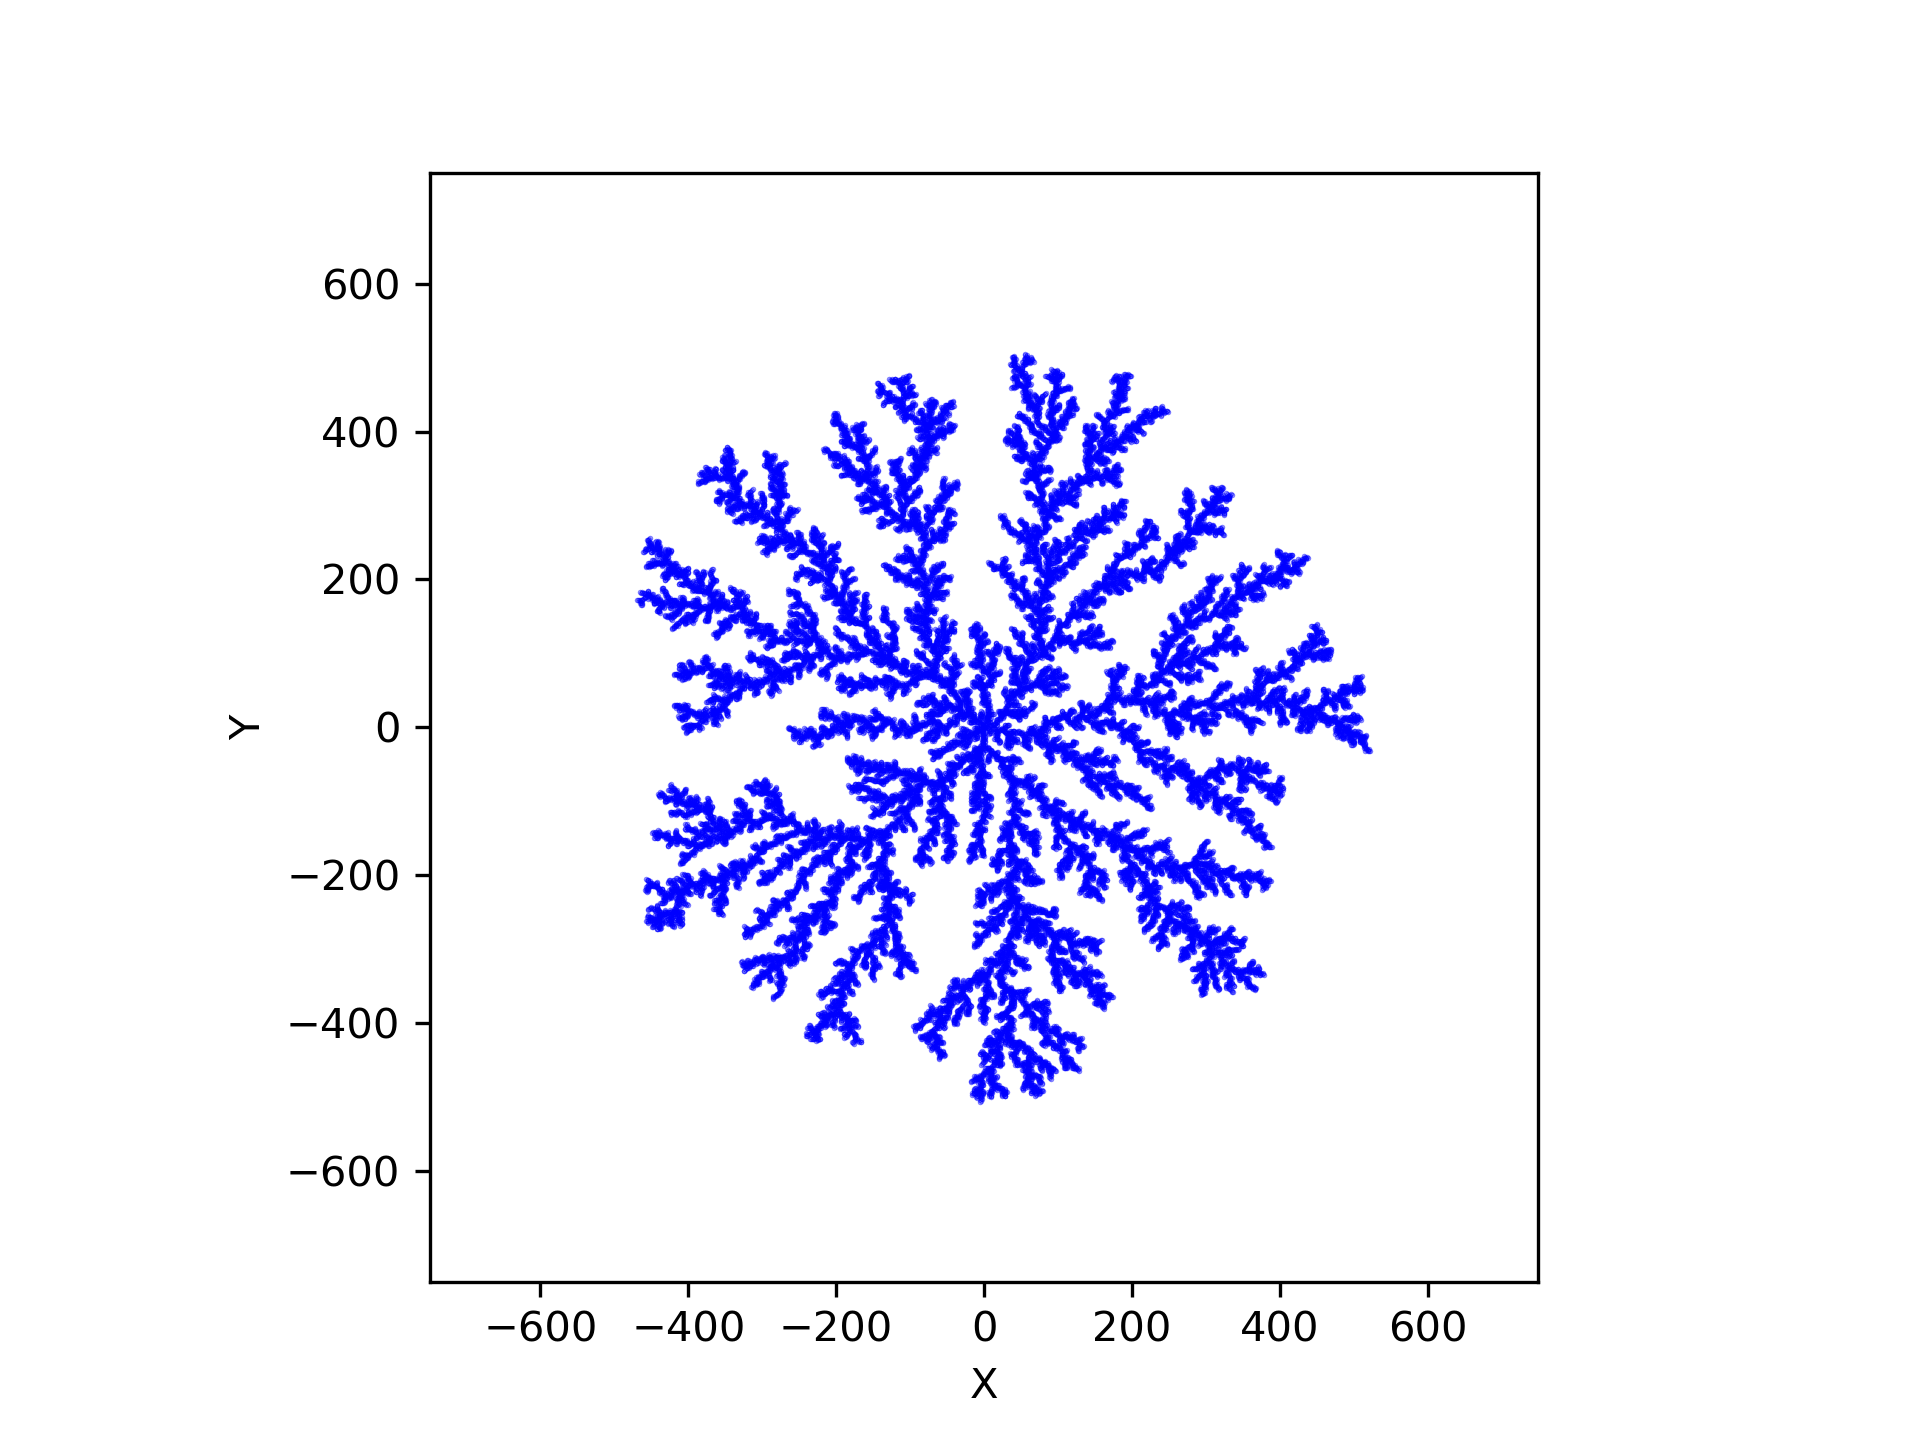
\includegraphics[width = 10cm]{改变max/1500-5*104-5-2*min.png}    
\caption{$R_{gen} = r_{cluster} + 5, R_{esp} = 2R_{gen}$的可视化模拟结果}    
\end{figure}

\newpage 修改逃逸边界半径为$2.5r_{cluster}$时有:

\begin{figure}[!htbp]        
\centering
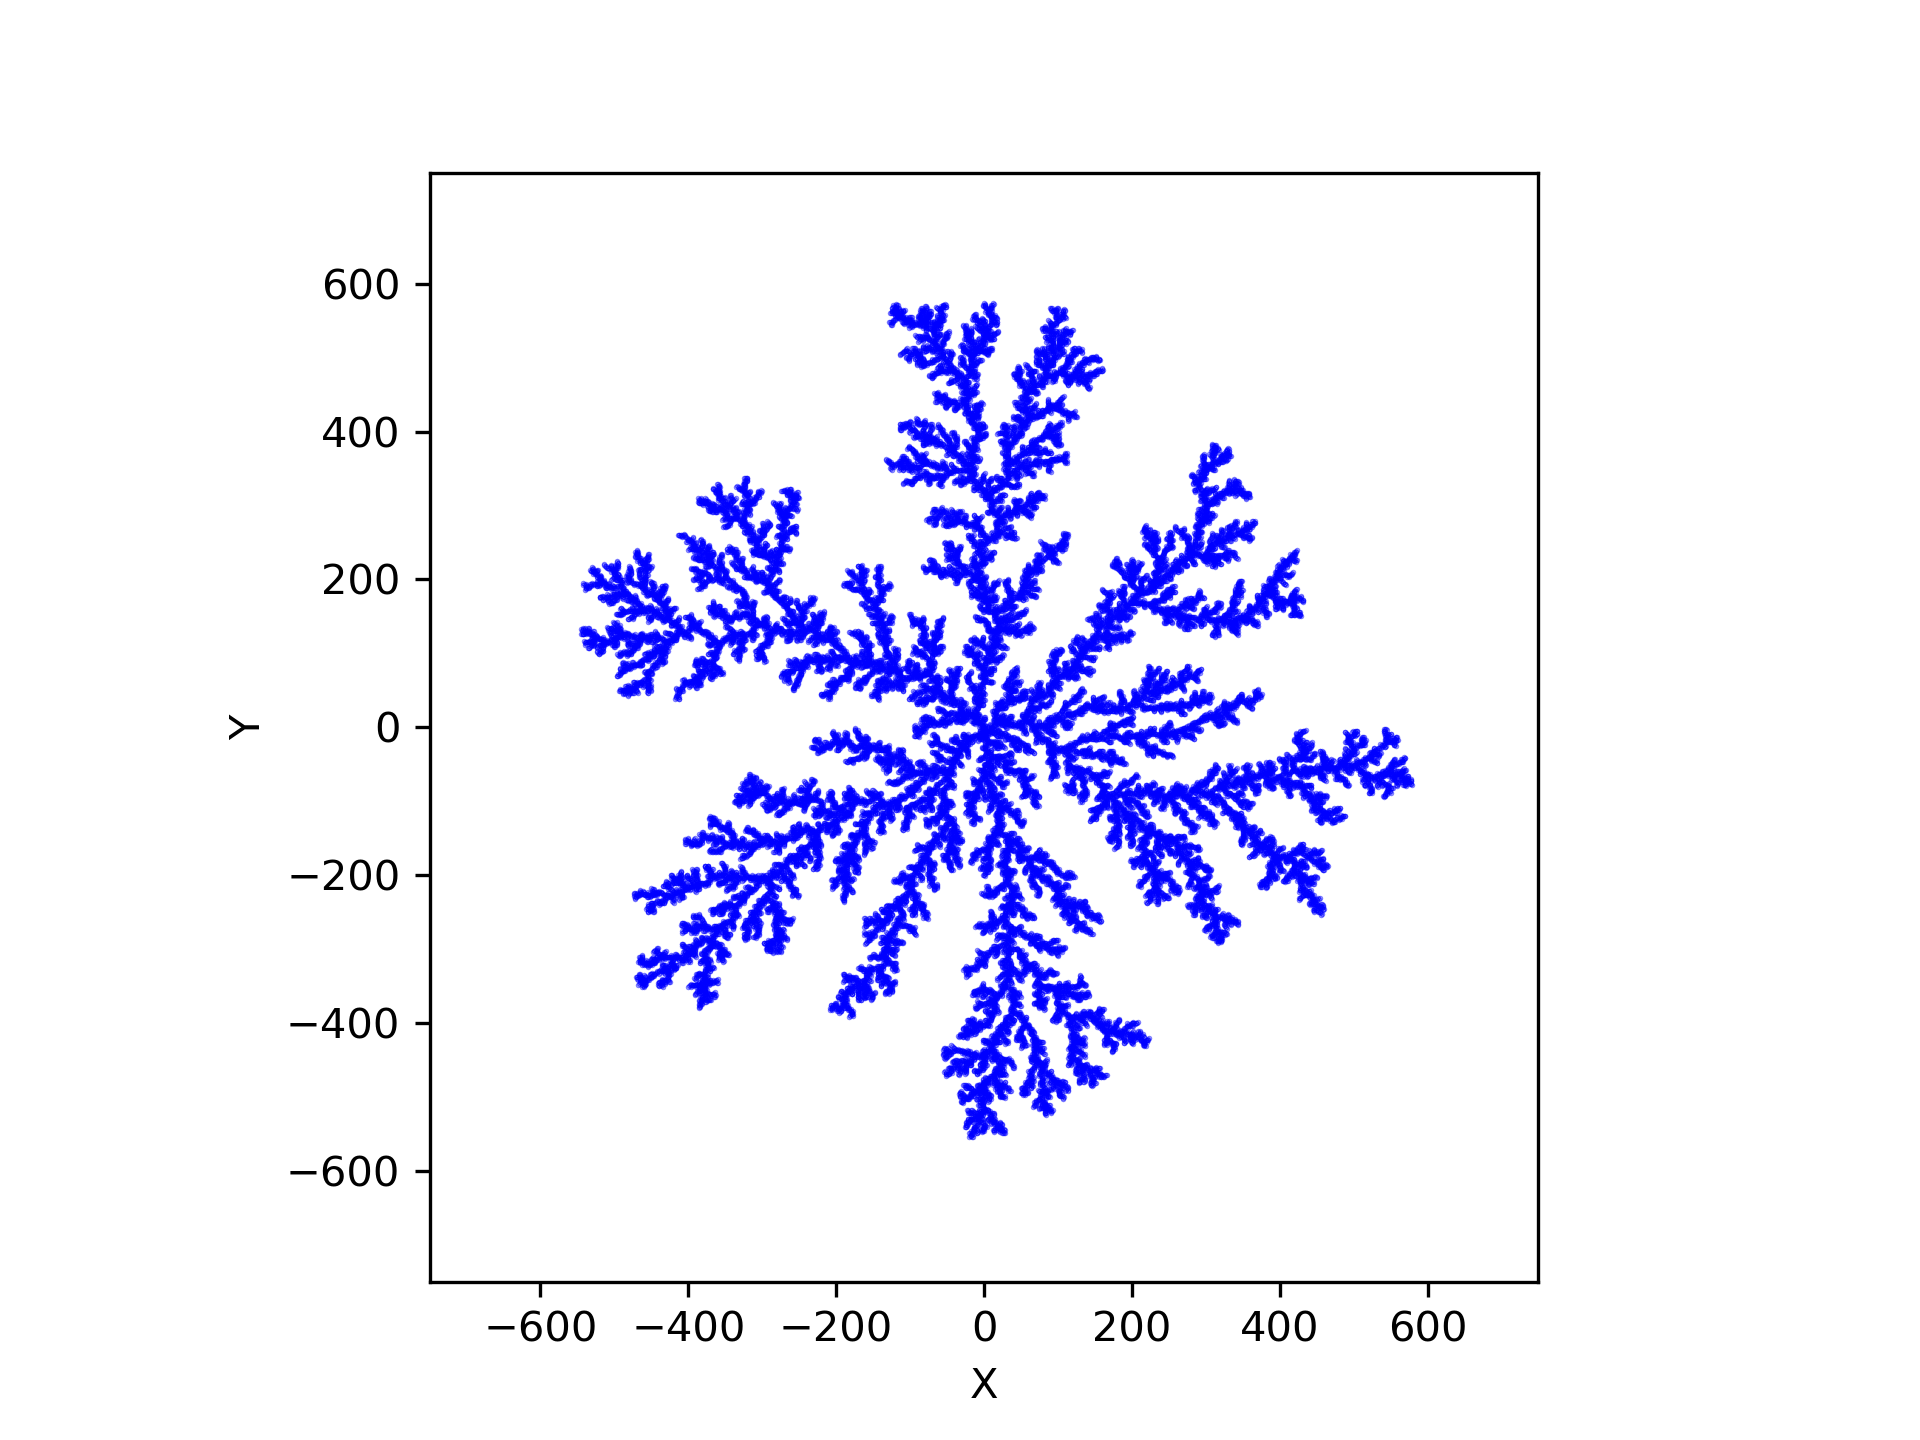
\includegraphics[bb= 0 0 460.8 345.6, width = 10cm]{改变max/1500-5*104-5-2.5*min.png}     
\caption{$R_{gen} = r_{cluster} + 5, R_{esp} = 2.5R_{gen}$的可视化模拟结果}      
\end{figure}

修改逃逸边界半径为$3r_{cluster}$时有:


\begin{figure}[!htbp]        
\centering
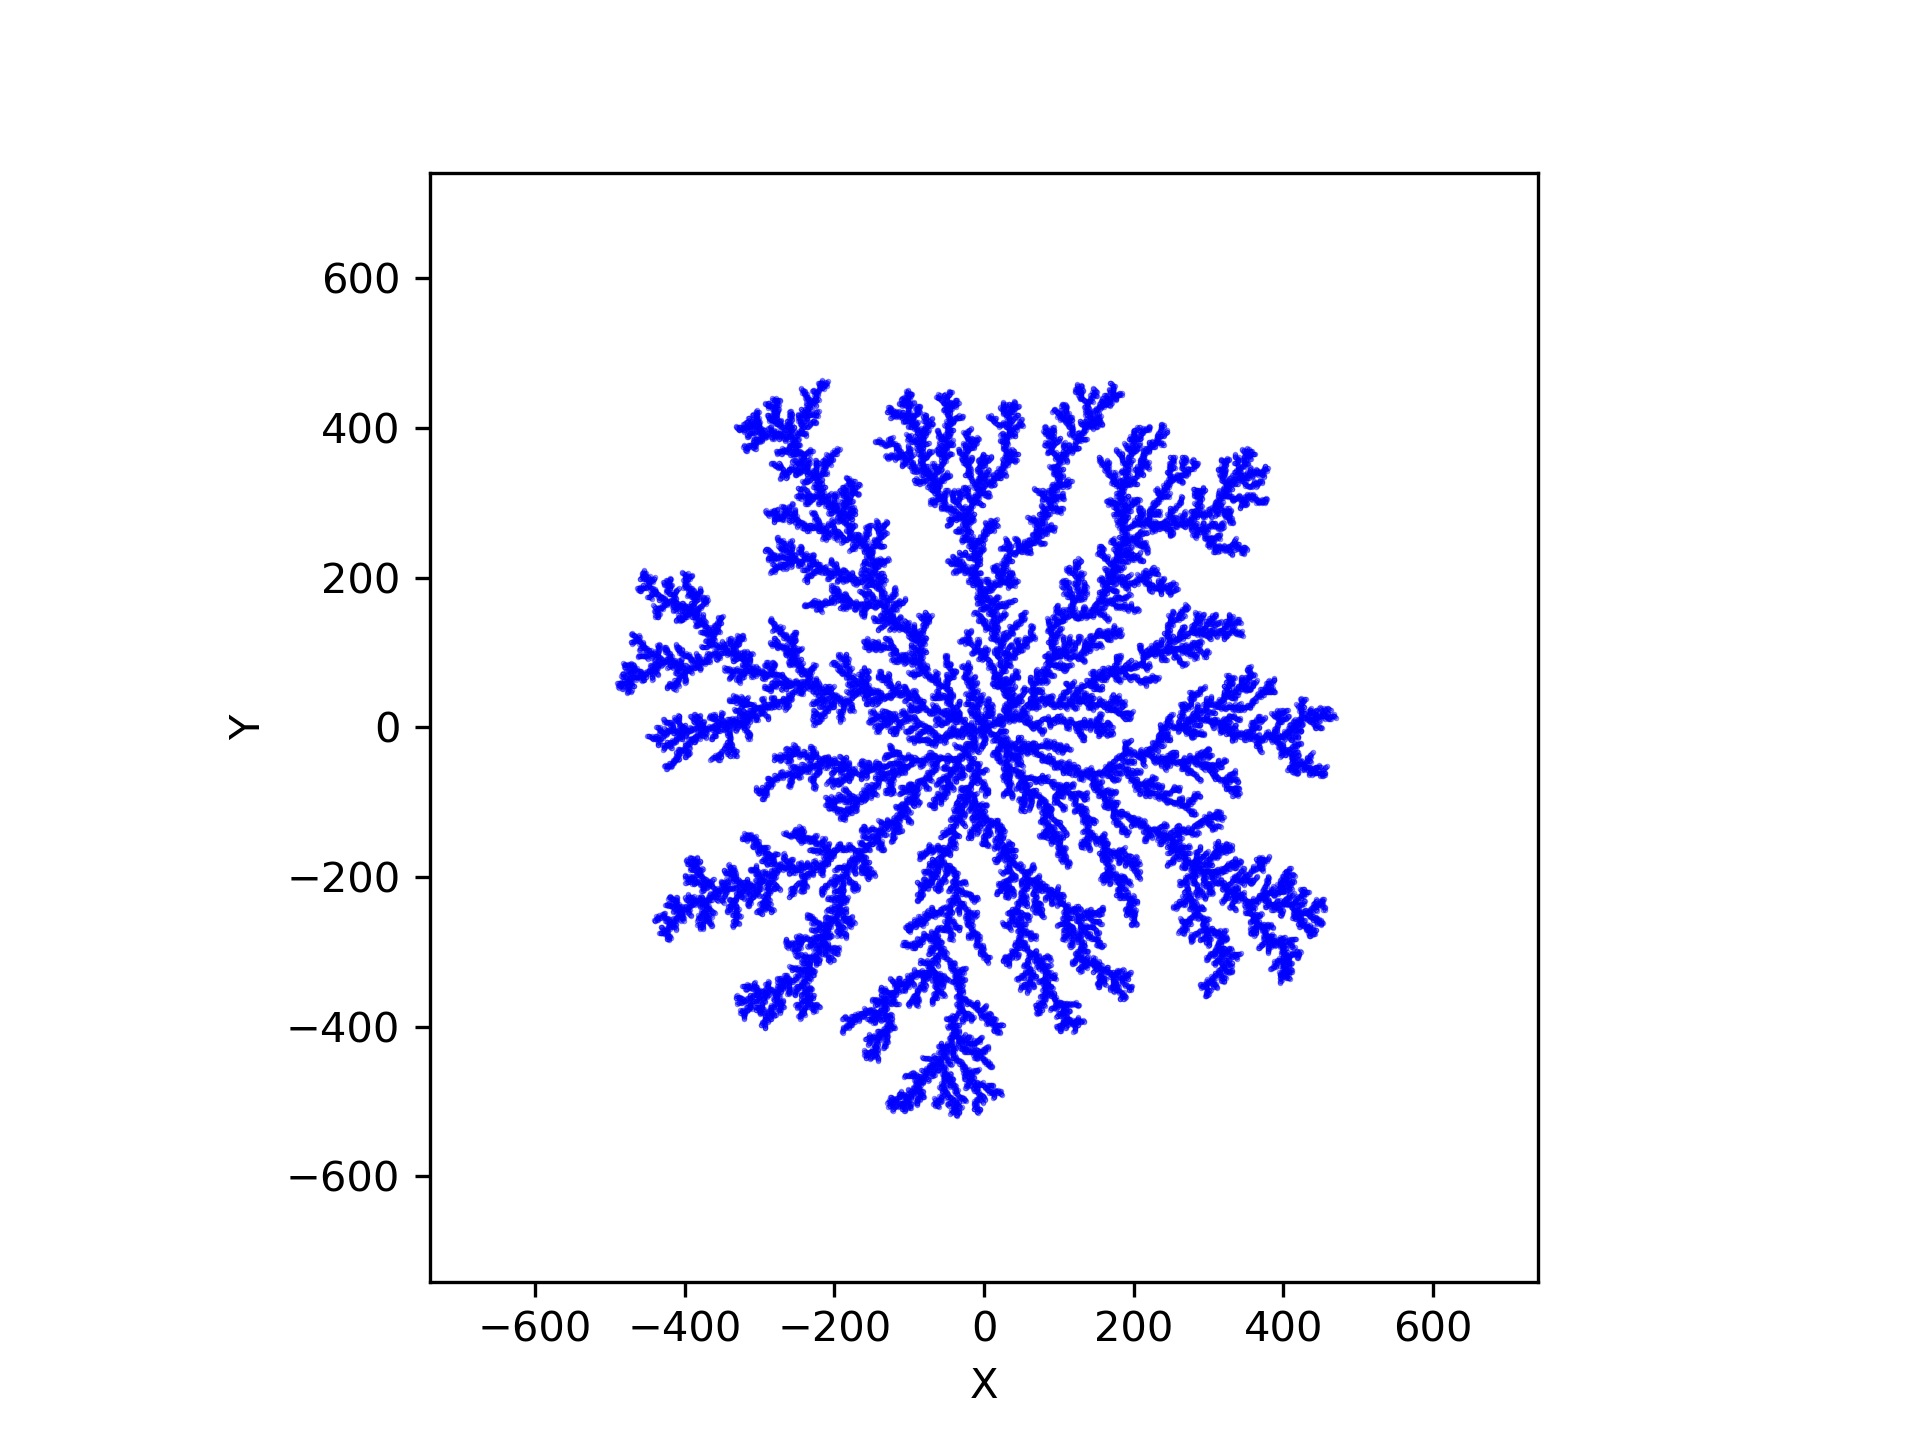
\includegraphics[bb= 0 0 460.8 345.6, width = 10cm]{改变max/2000-5*104-5-3*min.png}      
\caption{$R_{gen} = r_{cluster} + 5, R_{esp} = 3R_{gen}$的可视化模拟结果}      
\end{figure}


\newpage
可以看出三种逃逸边界的半径之间基本没有什么不同。


\subsection{分形维数计算}
对每个半径生成的数据做合计数法和Sandbox计数分别得到$lnN-ln(1/\epsilon)$和$lnN-lnr$的散点图,线性拟合得到的斜率即为数值模拟得到的分形维数。有如下结果:


\begin{figure}[!htbp]   
\centering     
\subfigure[盒计数法]{
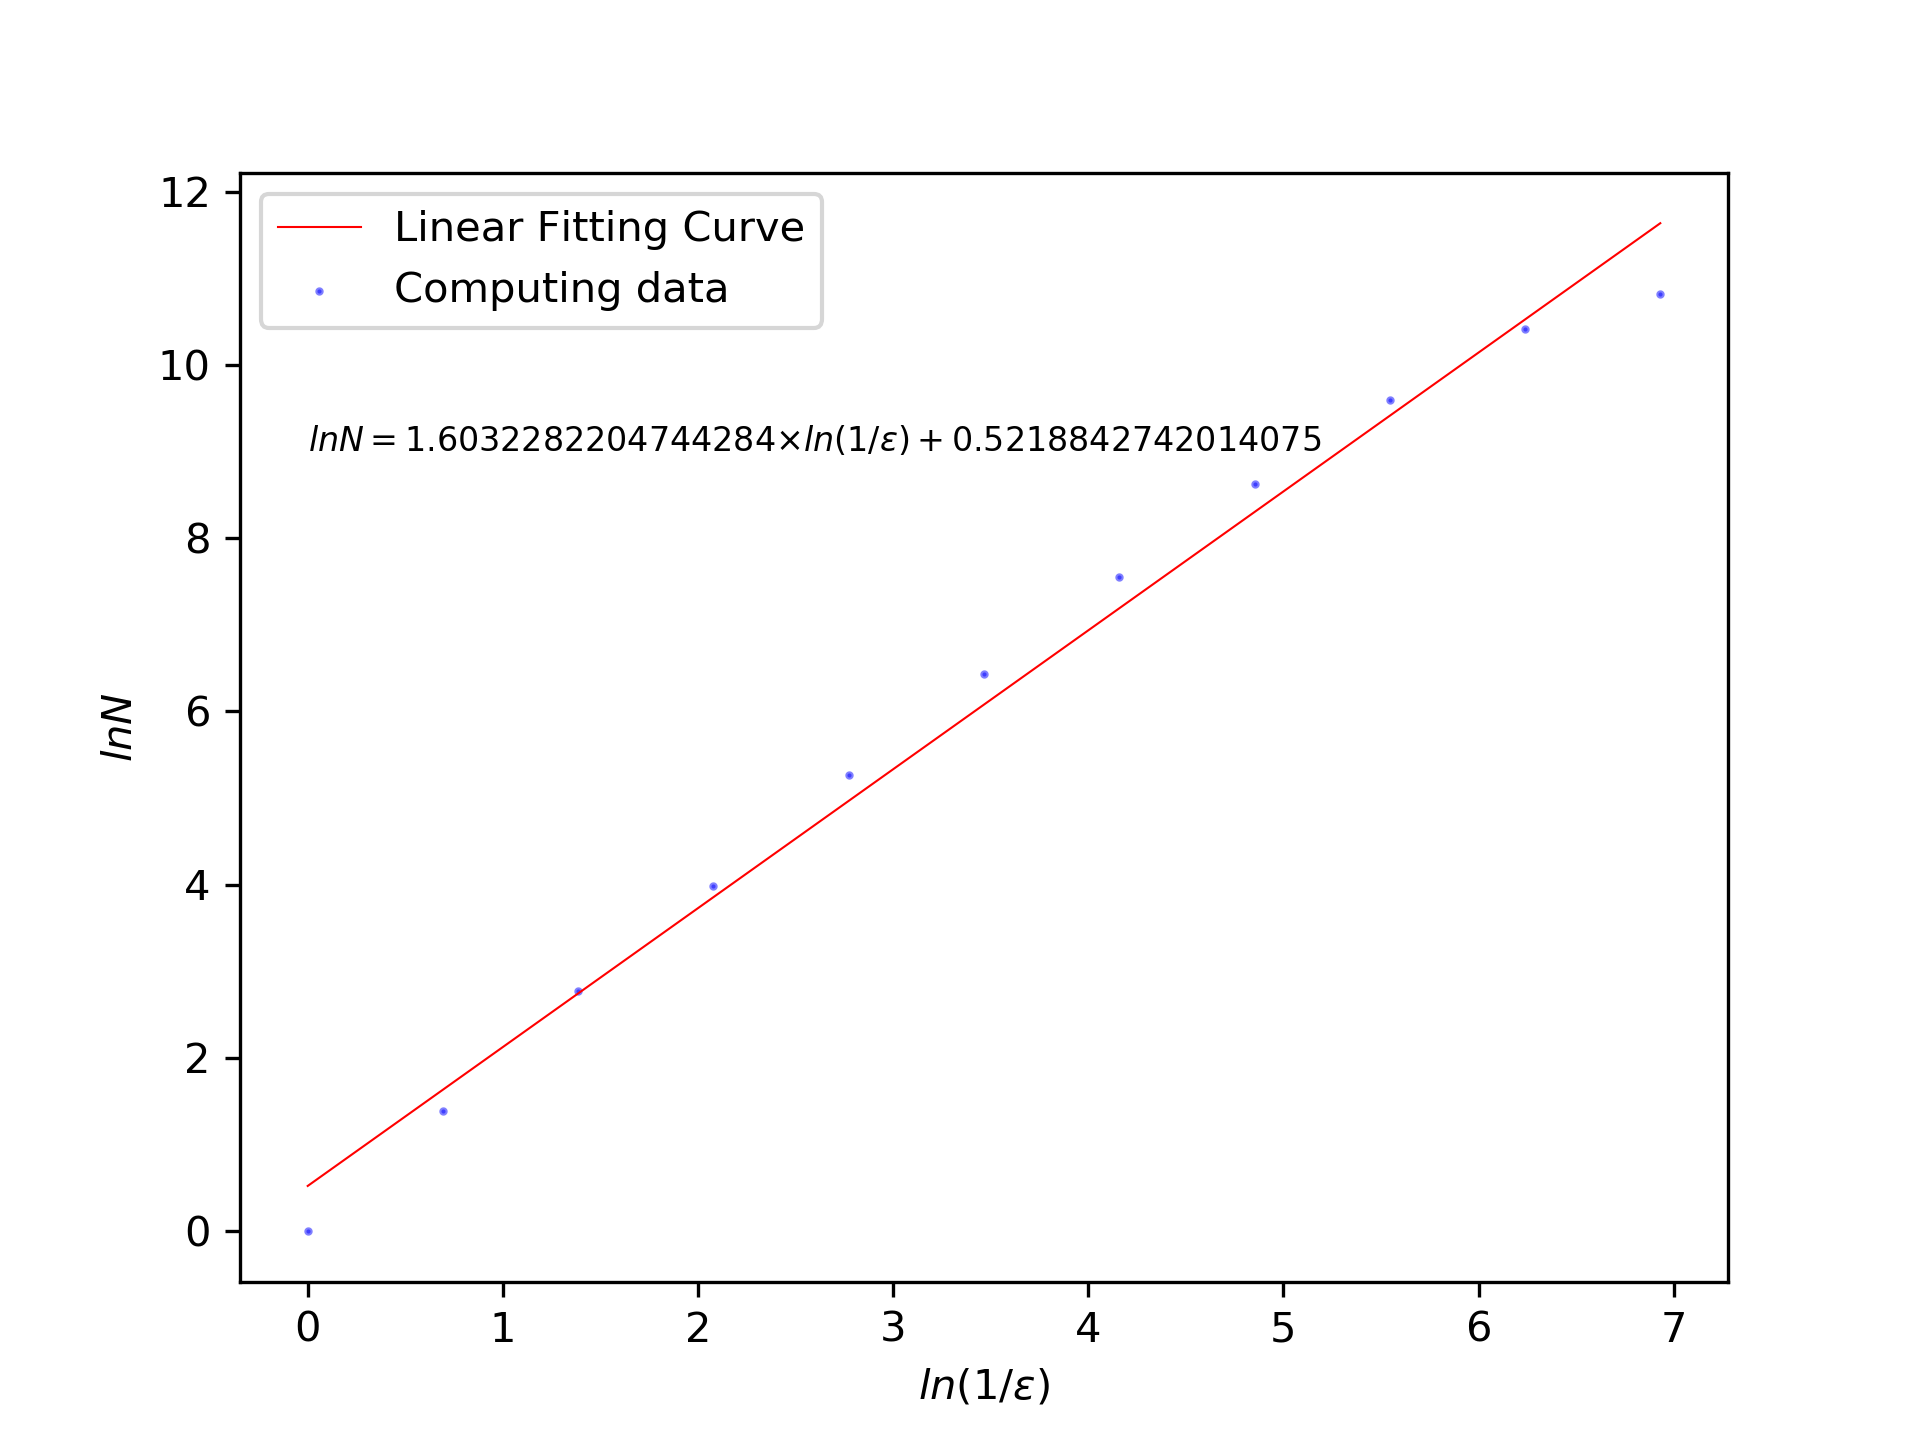
\includegraphics[width=6cm] {分形维数/box-5-2*min.png}
}
\subfigure[Sandbox法]{
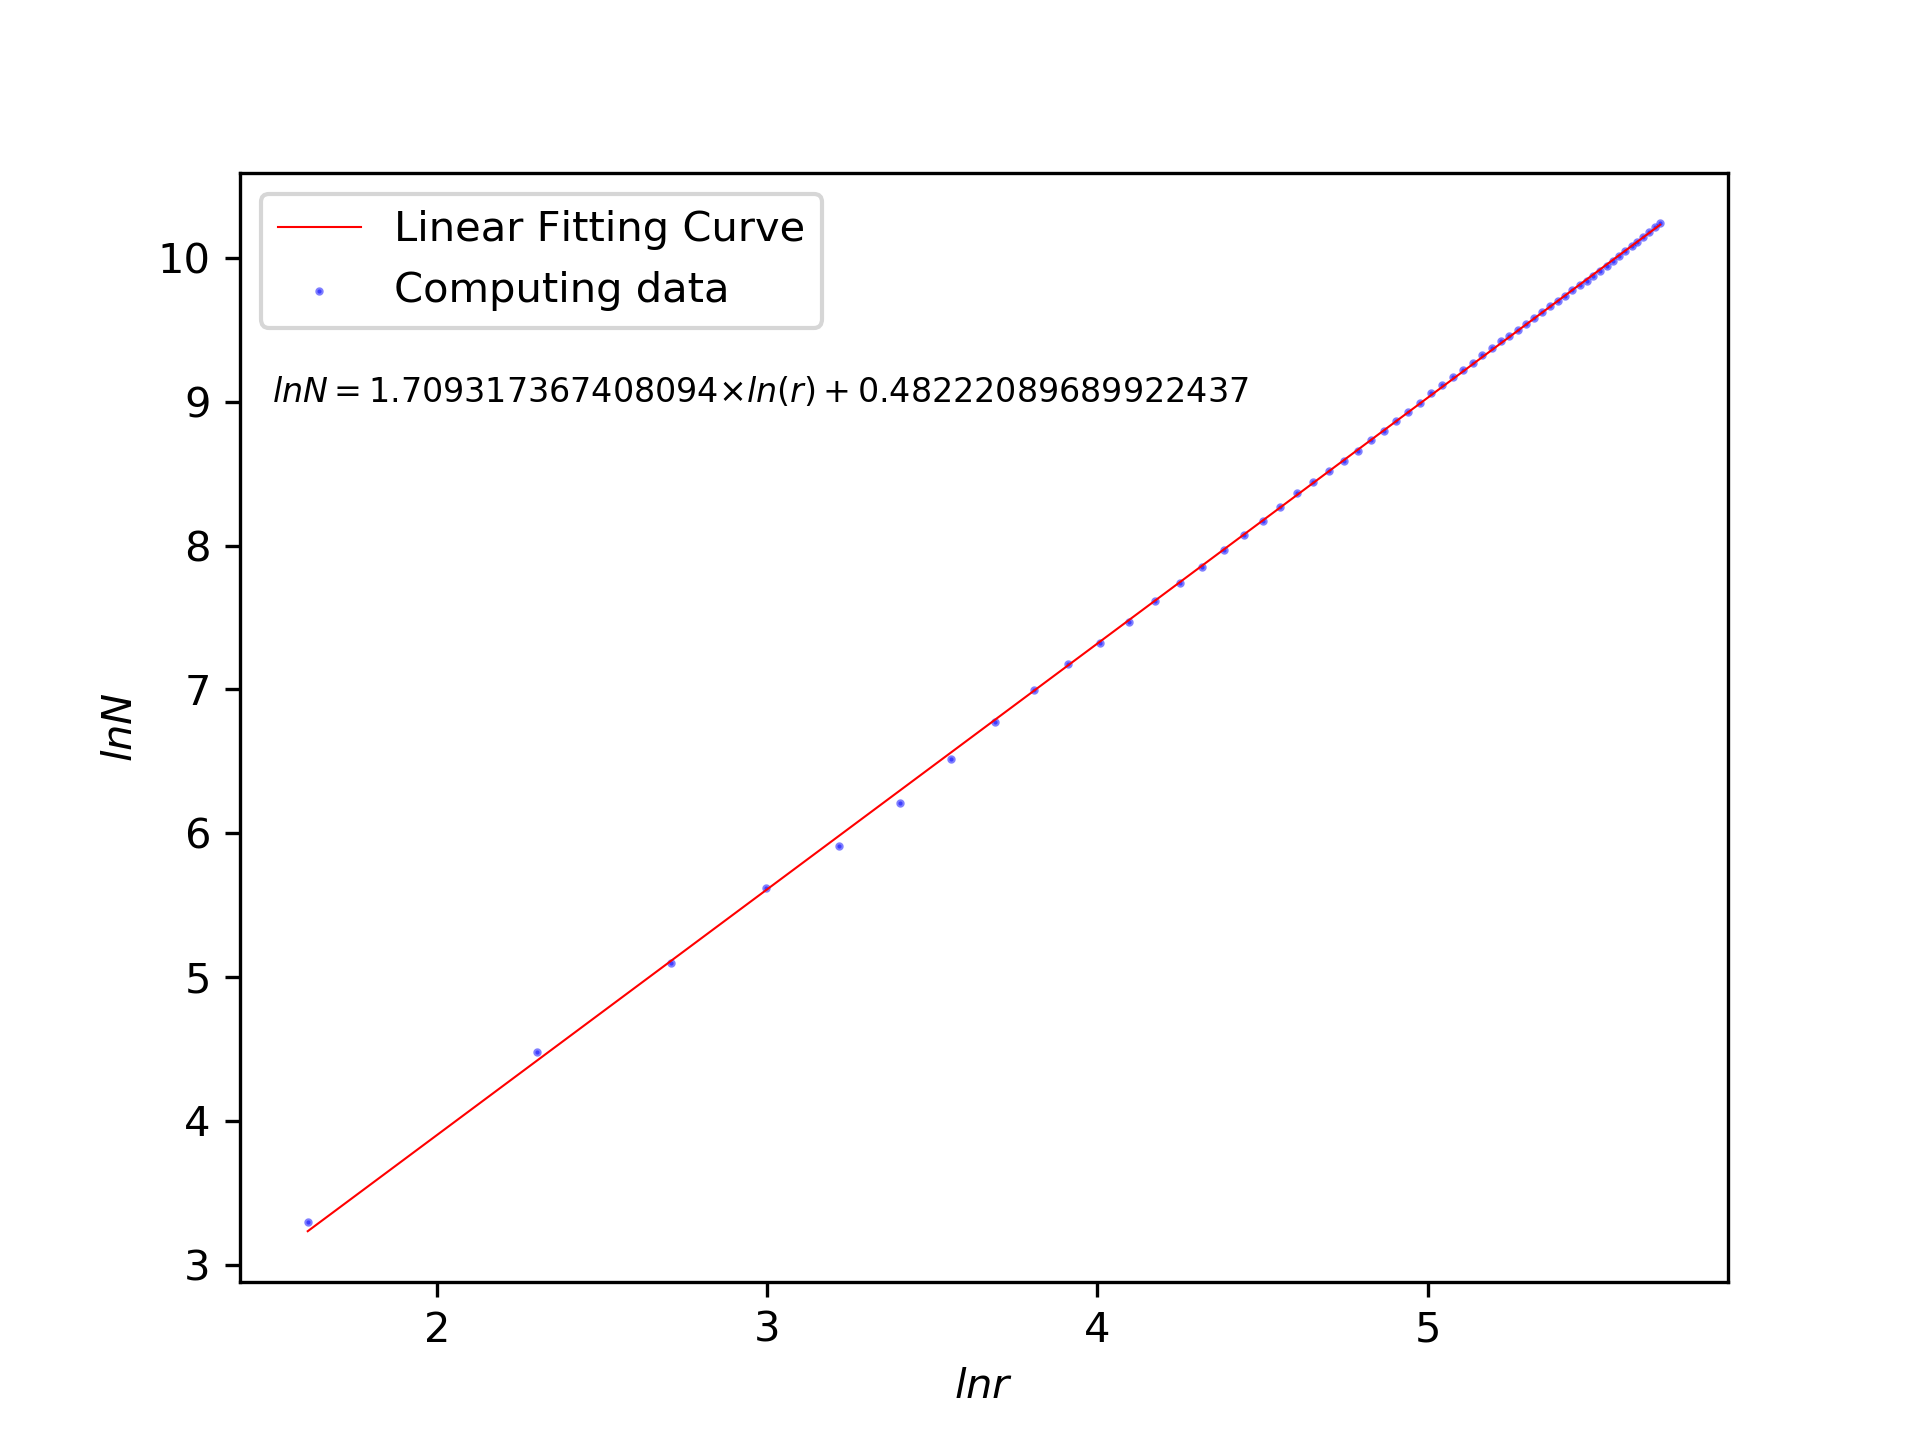
\includegraphics[width=6cm] {分形维数/sandbox-5-2*min.png}
}            
\caption{$R_{gen} = r_{cluster} + 5, R_{esp} = 2R_{gen}$的分形维数计算}      
\end{figure}


\begin{figure}[!htbp]   
\centering     
\subfigure[盒计数法]{
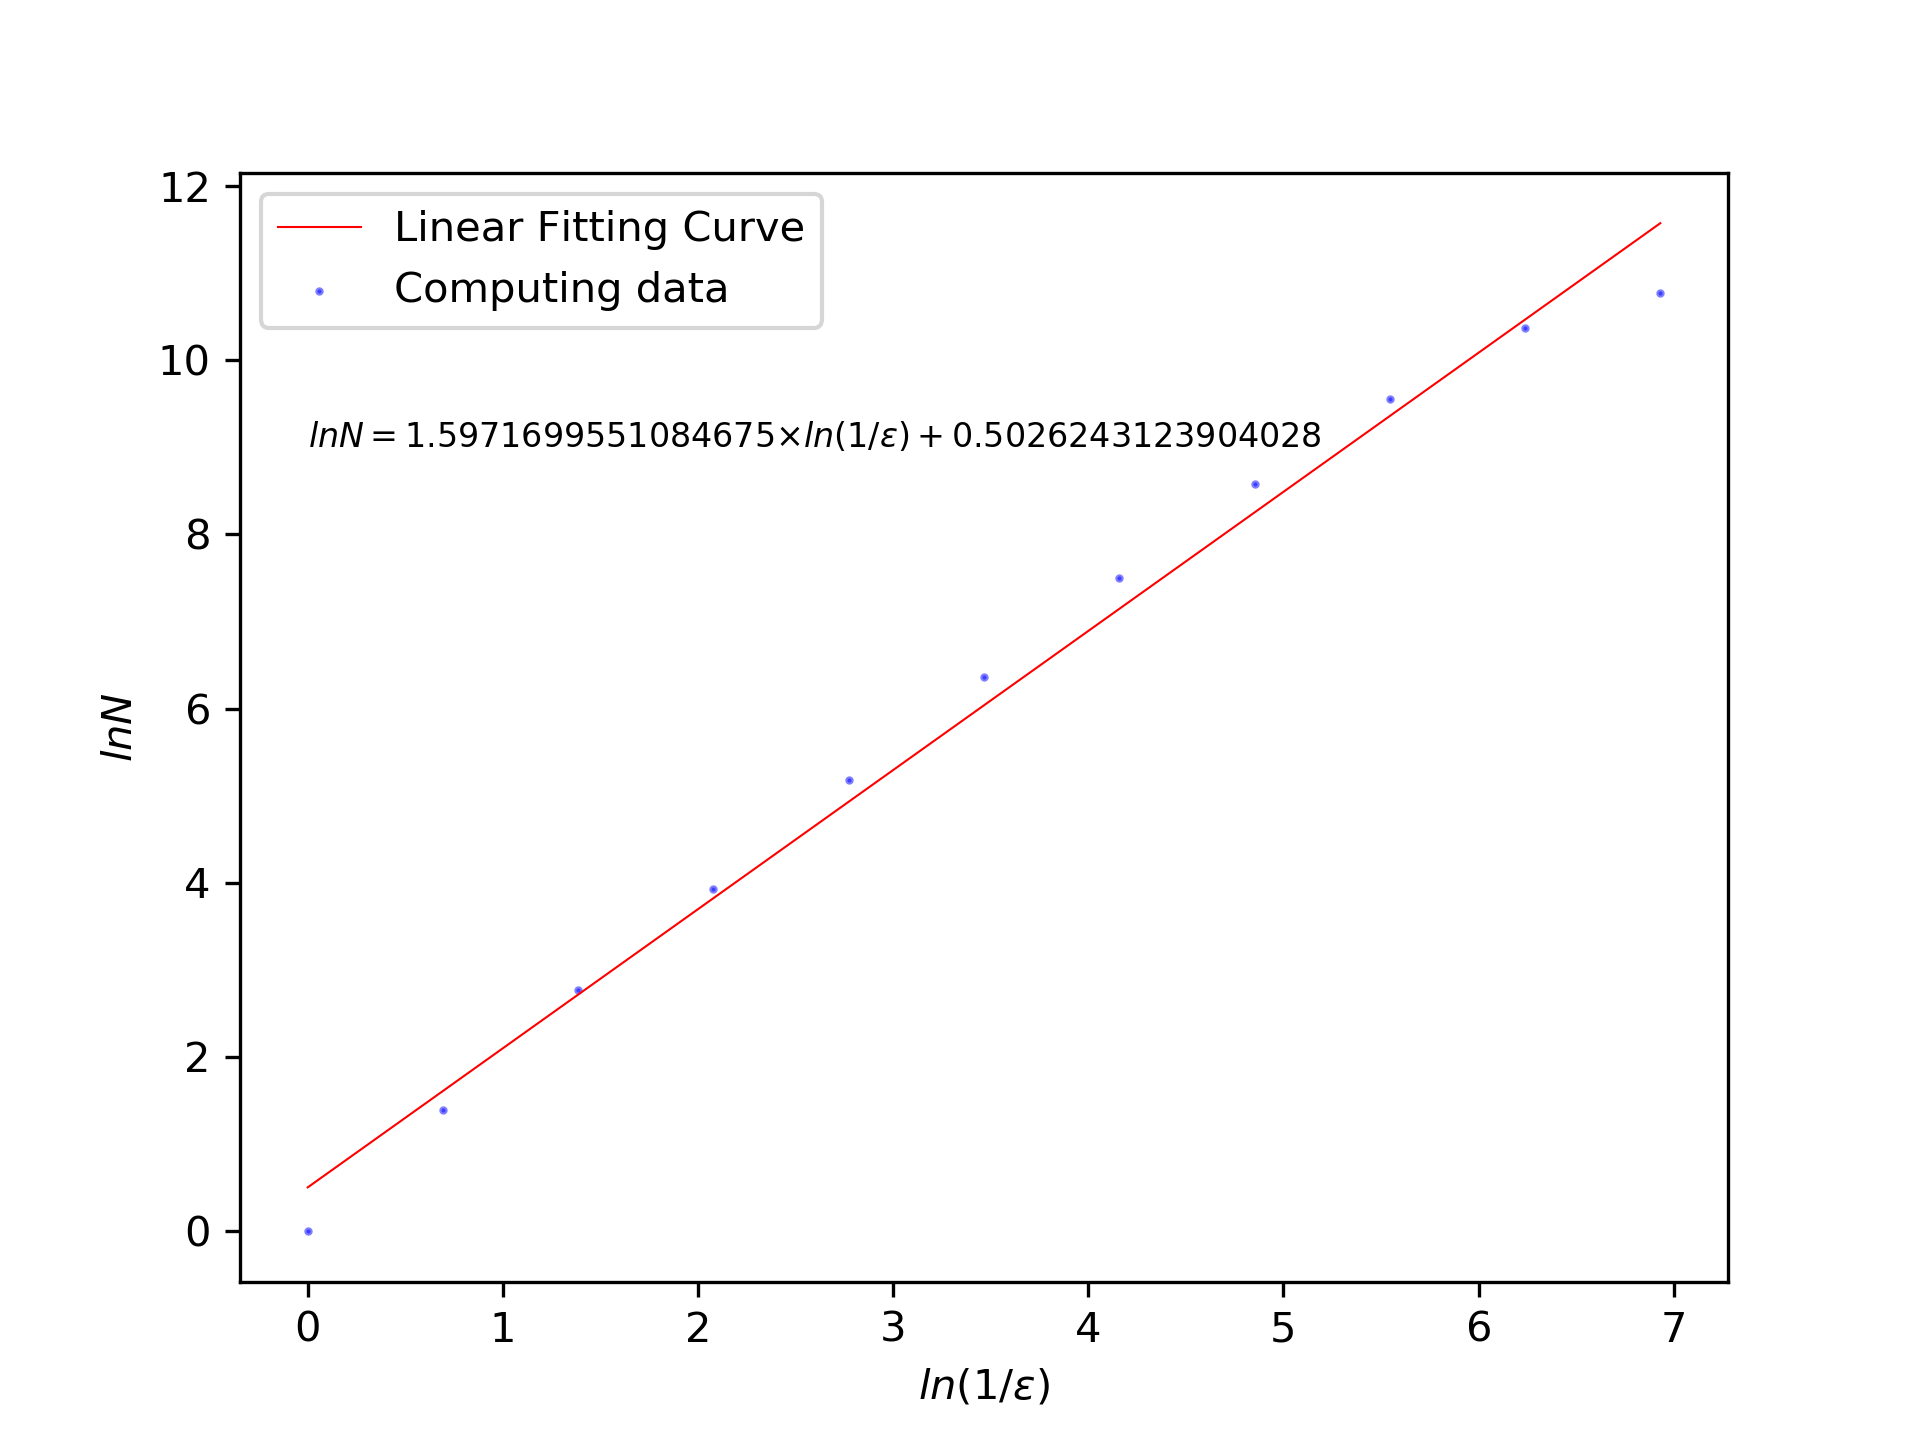
\includegraphics[bb= 0 0 460.8 345.6,width=6cm] {分形维数/box-5-2.5*min.png}
}
\subfigure[Sandbox法]{
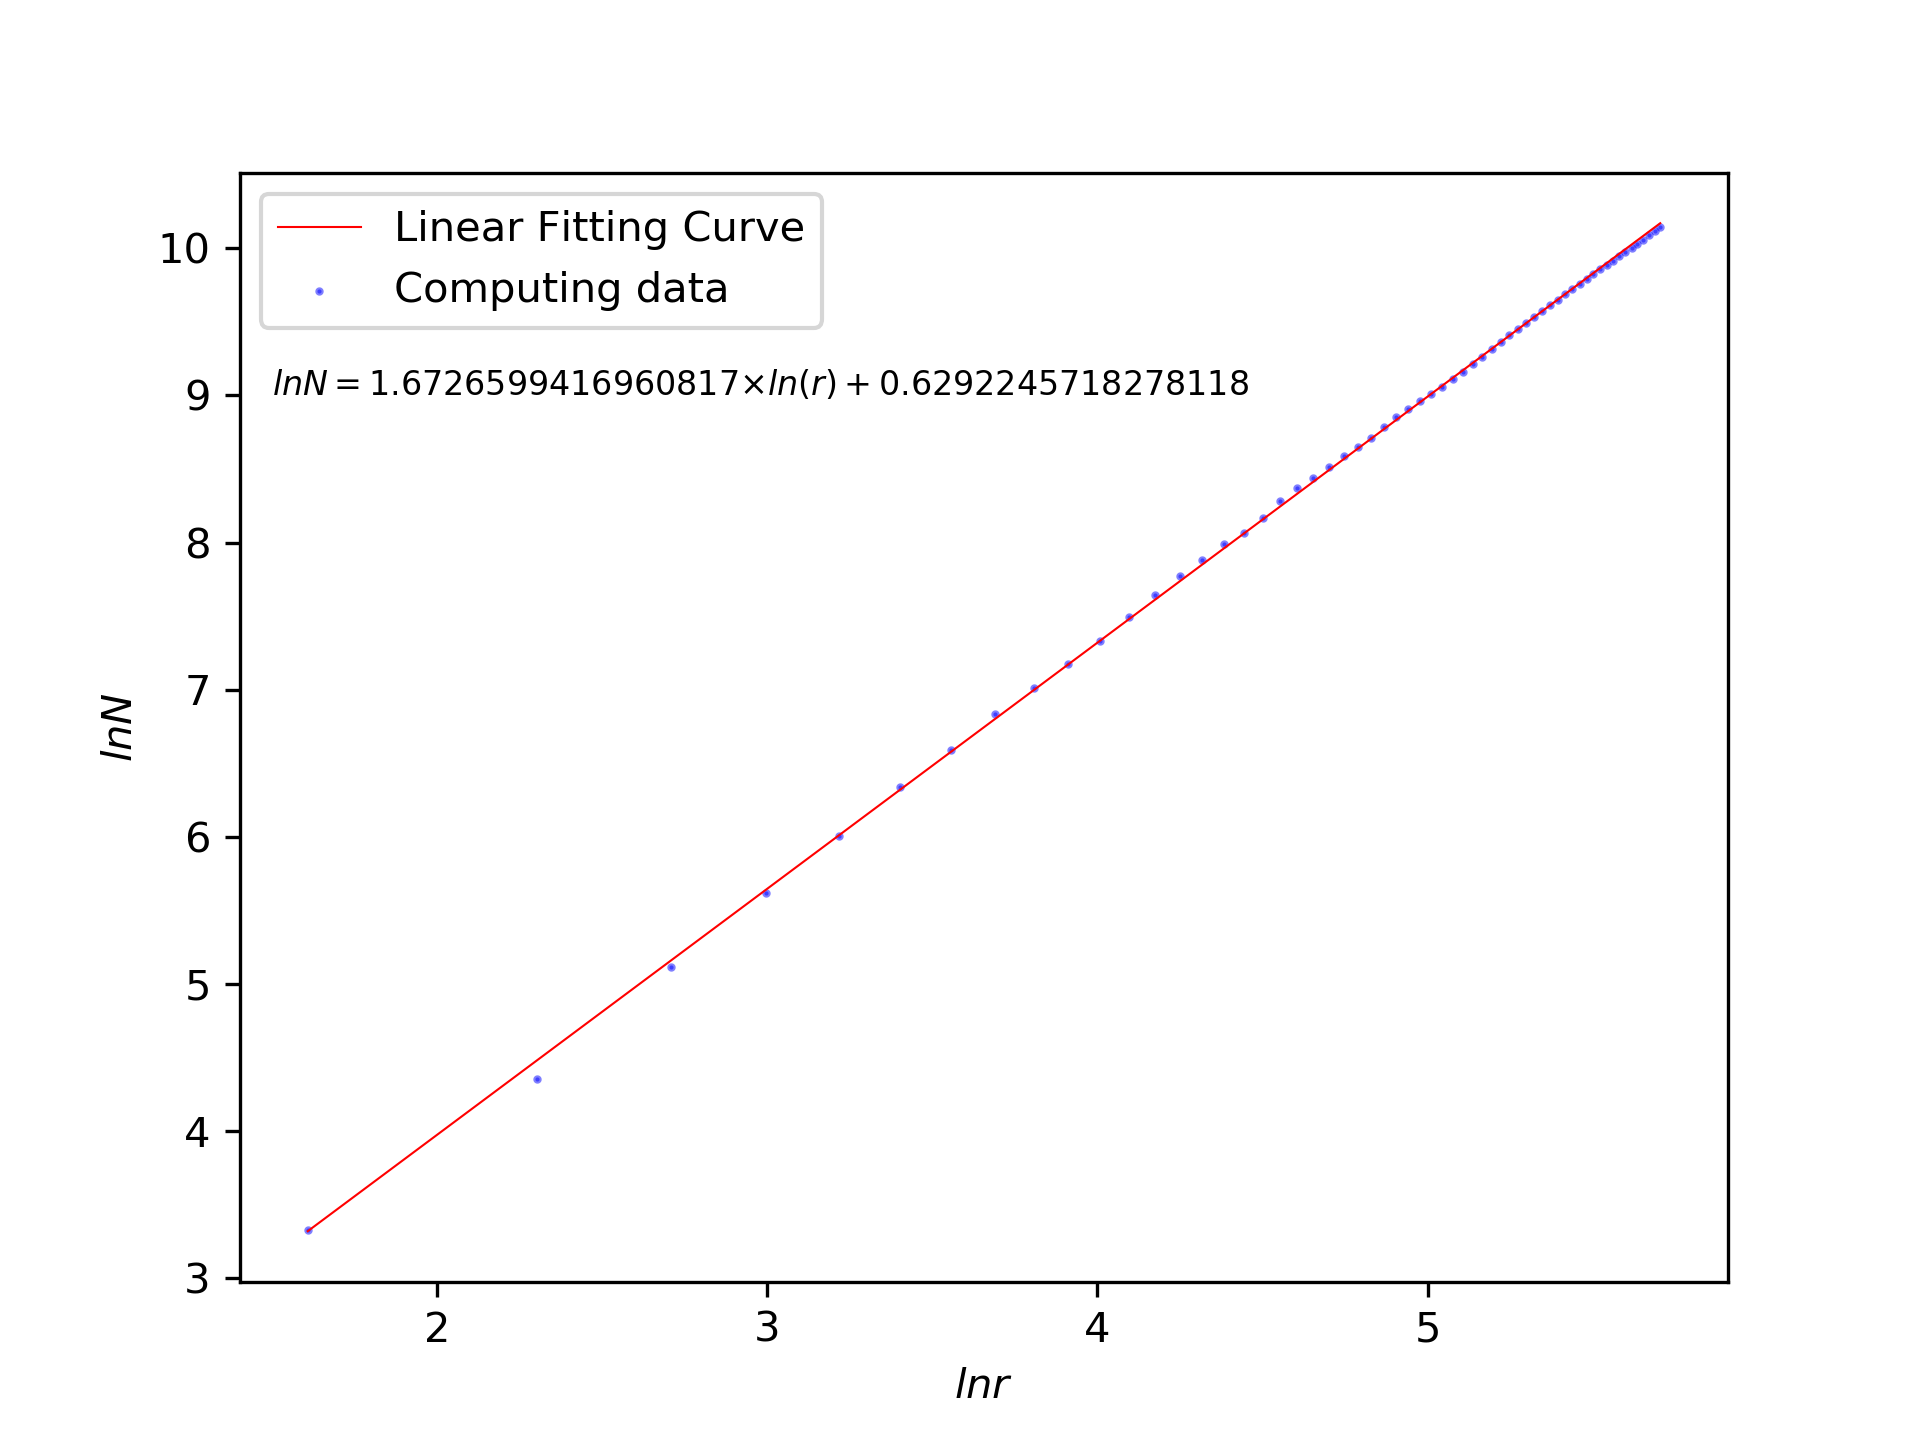
\includegraphics[bb= 0 0 460.8 345.6,width=6cm] {分形维数/sandbox-5-2.5*min.png}
}            
\caption{$R_{gen} = r_{cluster} + 5, R_{esp} = 2.5R_{gen}$的分形维数计算}      
\end{figure}


\begin{figure}[!htbp]   
\centering     
\subfigure[盒计数法]{
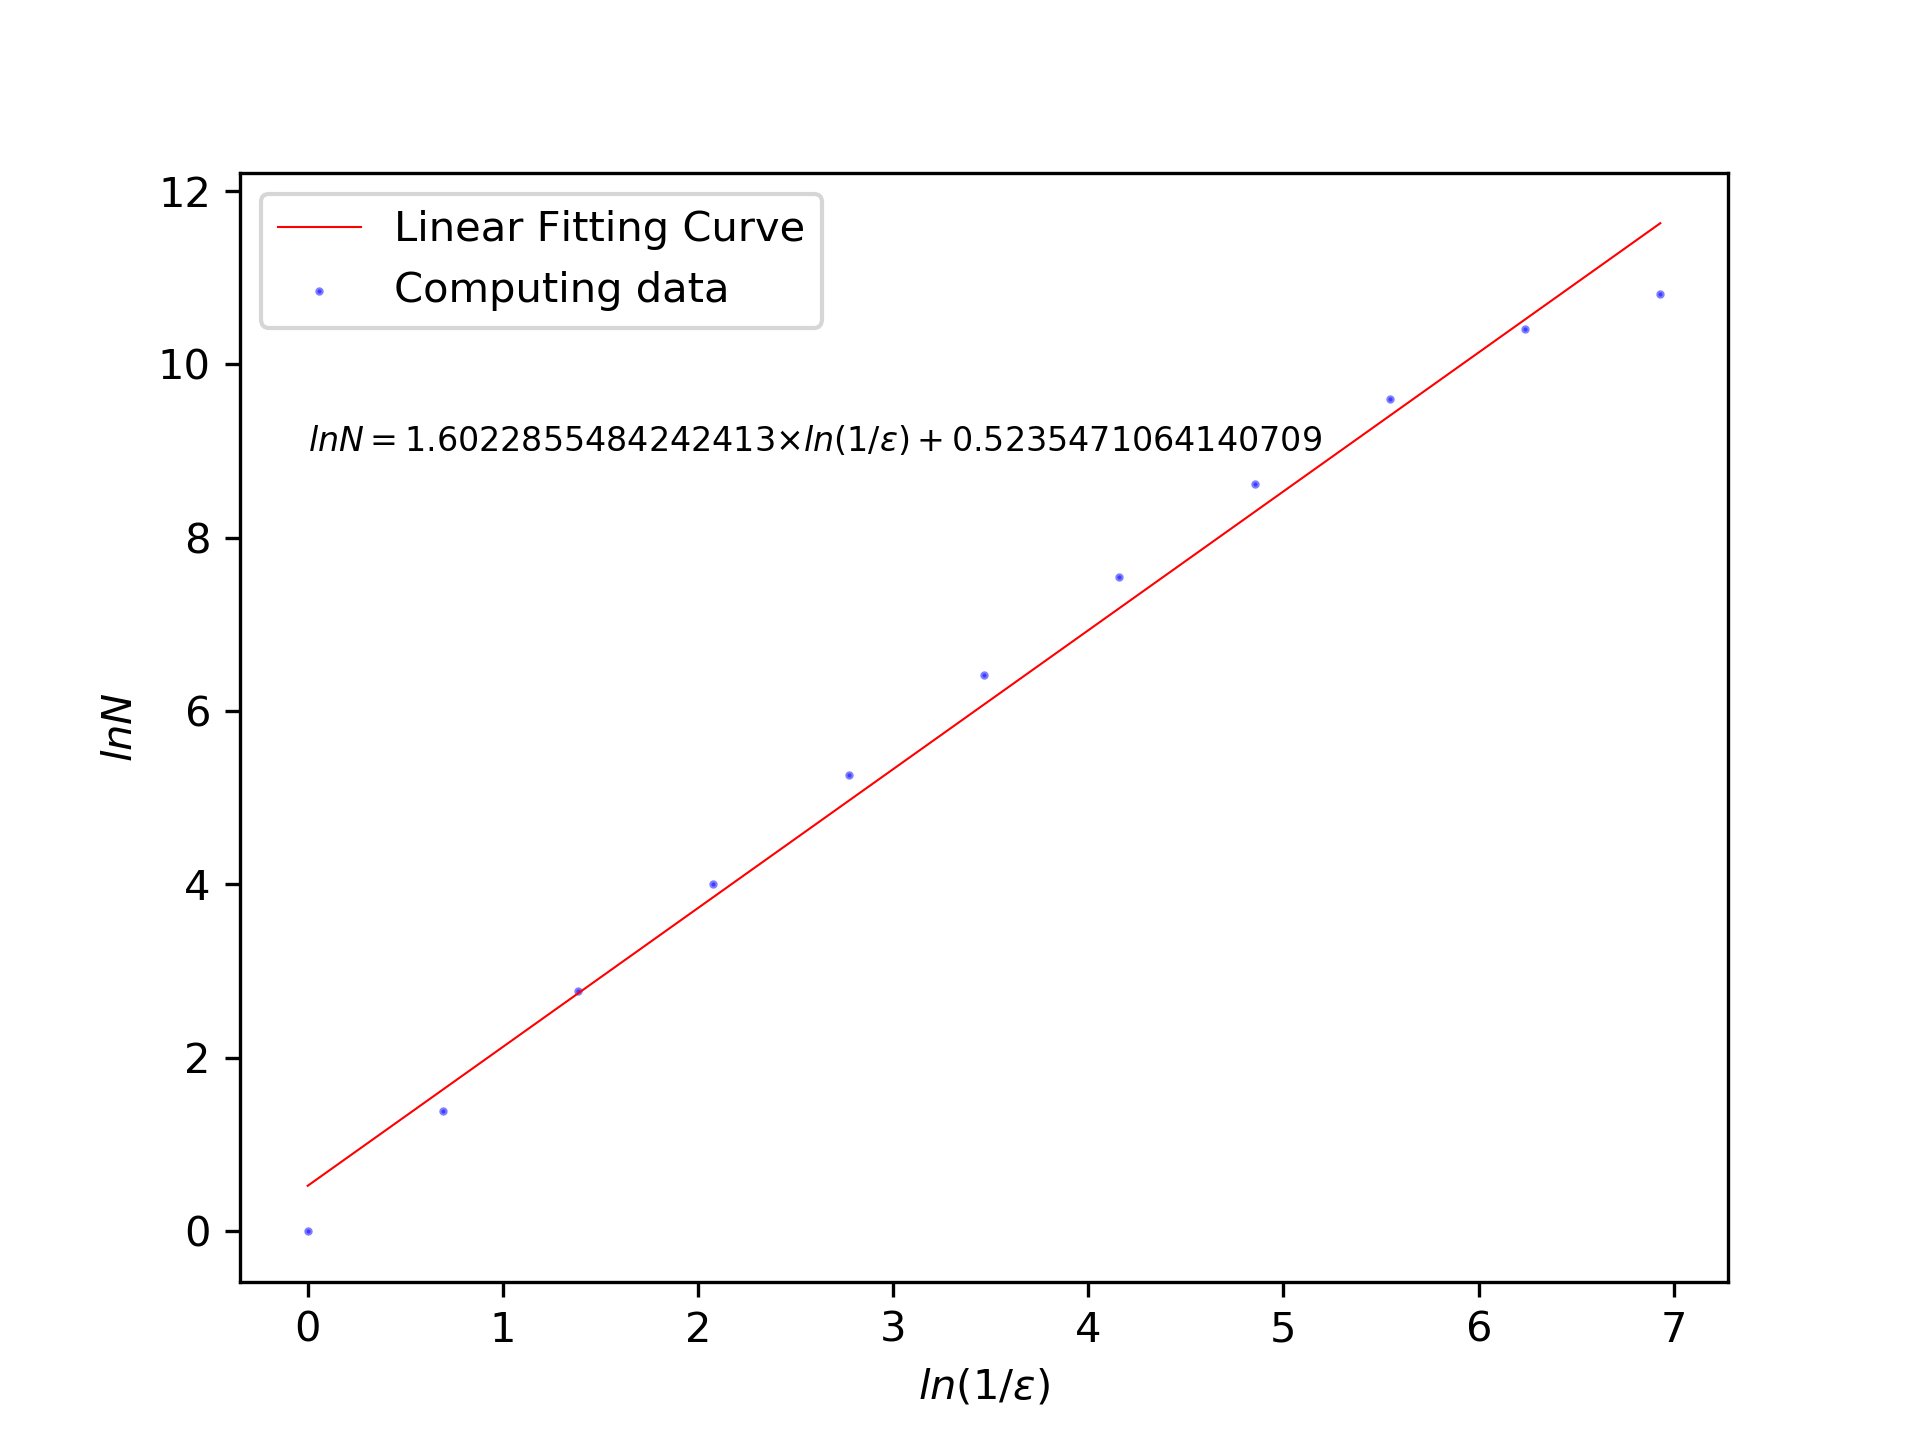
\includegraphics[width=6cm] {分形维数/box-5-3*min.png}
}
\subfigure[Sandbox法]{
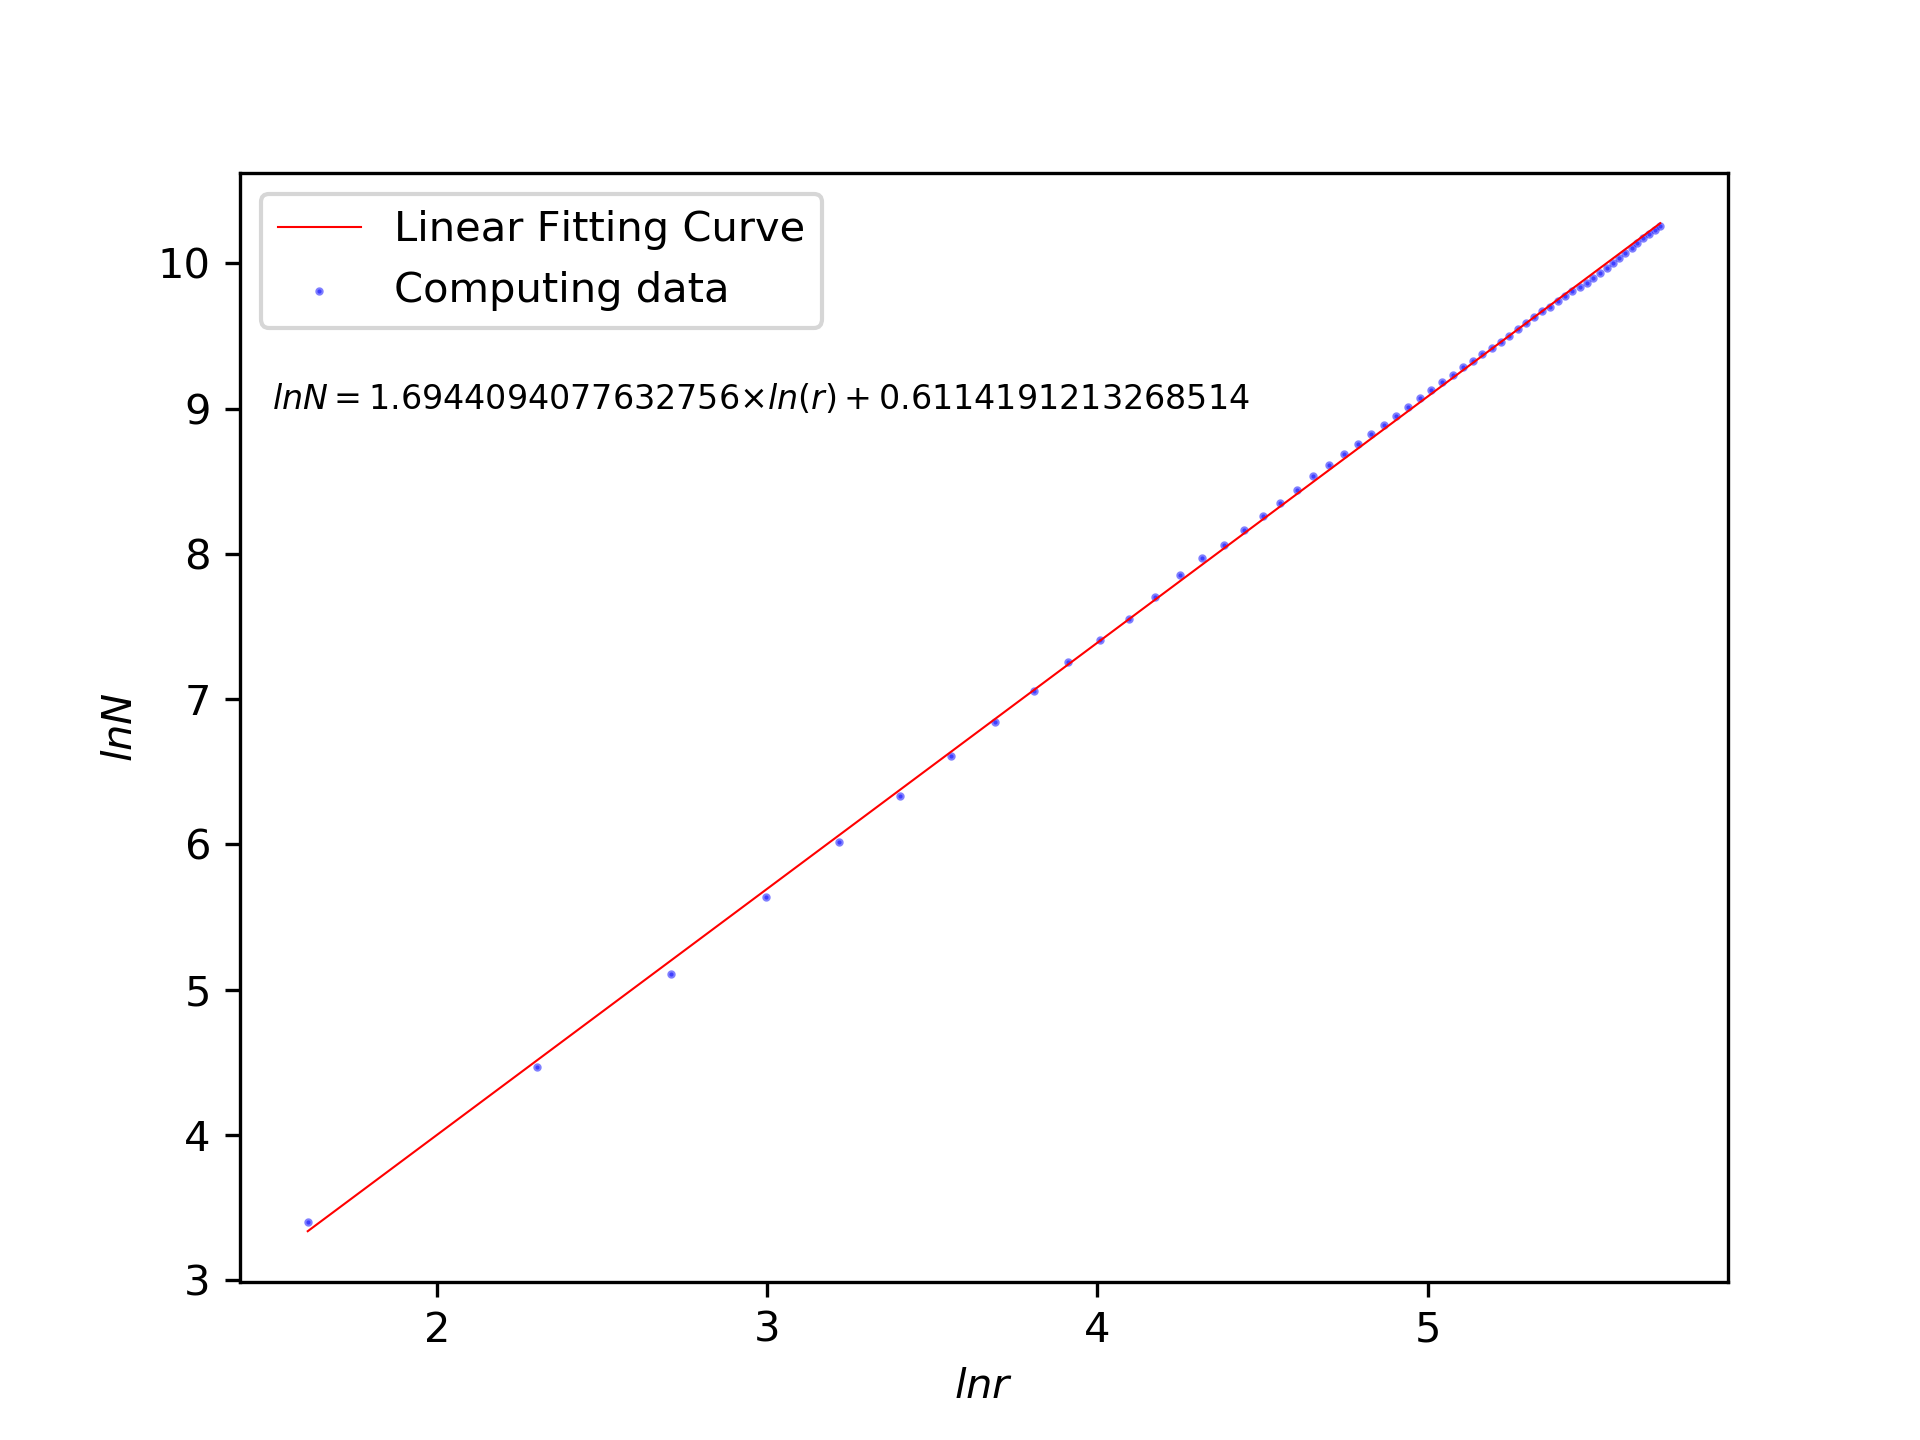
\includegraphics[width=6cm] {分形维数/sandbox-5-3*min.png}
}           
\caption{$R_{gen} = r_{cluster} + 5, R_{esp} = 3R_{gen}$的分形维数计算}      
\end{figure}


我们看到两个方法得到的分形维数还是有一些差异的,具体原因不知,可能由于盒计数法点数不够多,导致误差较大。可认为DLA的分形维数在$1.6-1.7$之间。有趣的是,我们能够看出对于盒计数法来说,最后一个点偏离拟合直线许多,于是我们认为删掉最后一个点的数据得到:

\begin{figure}[!htbp]        
\centering
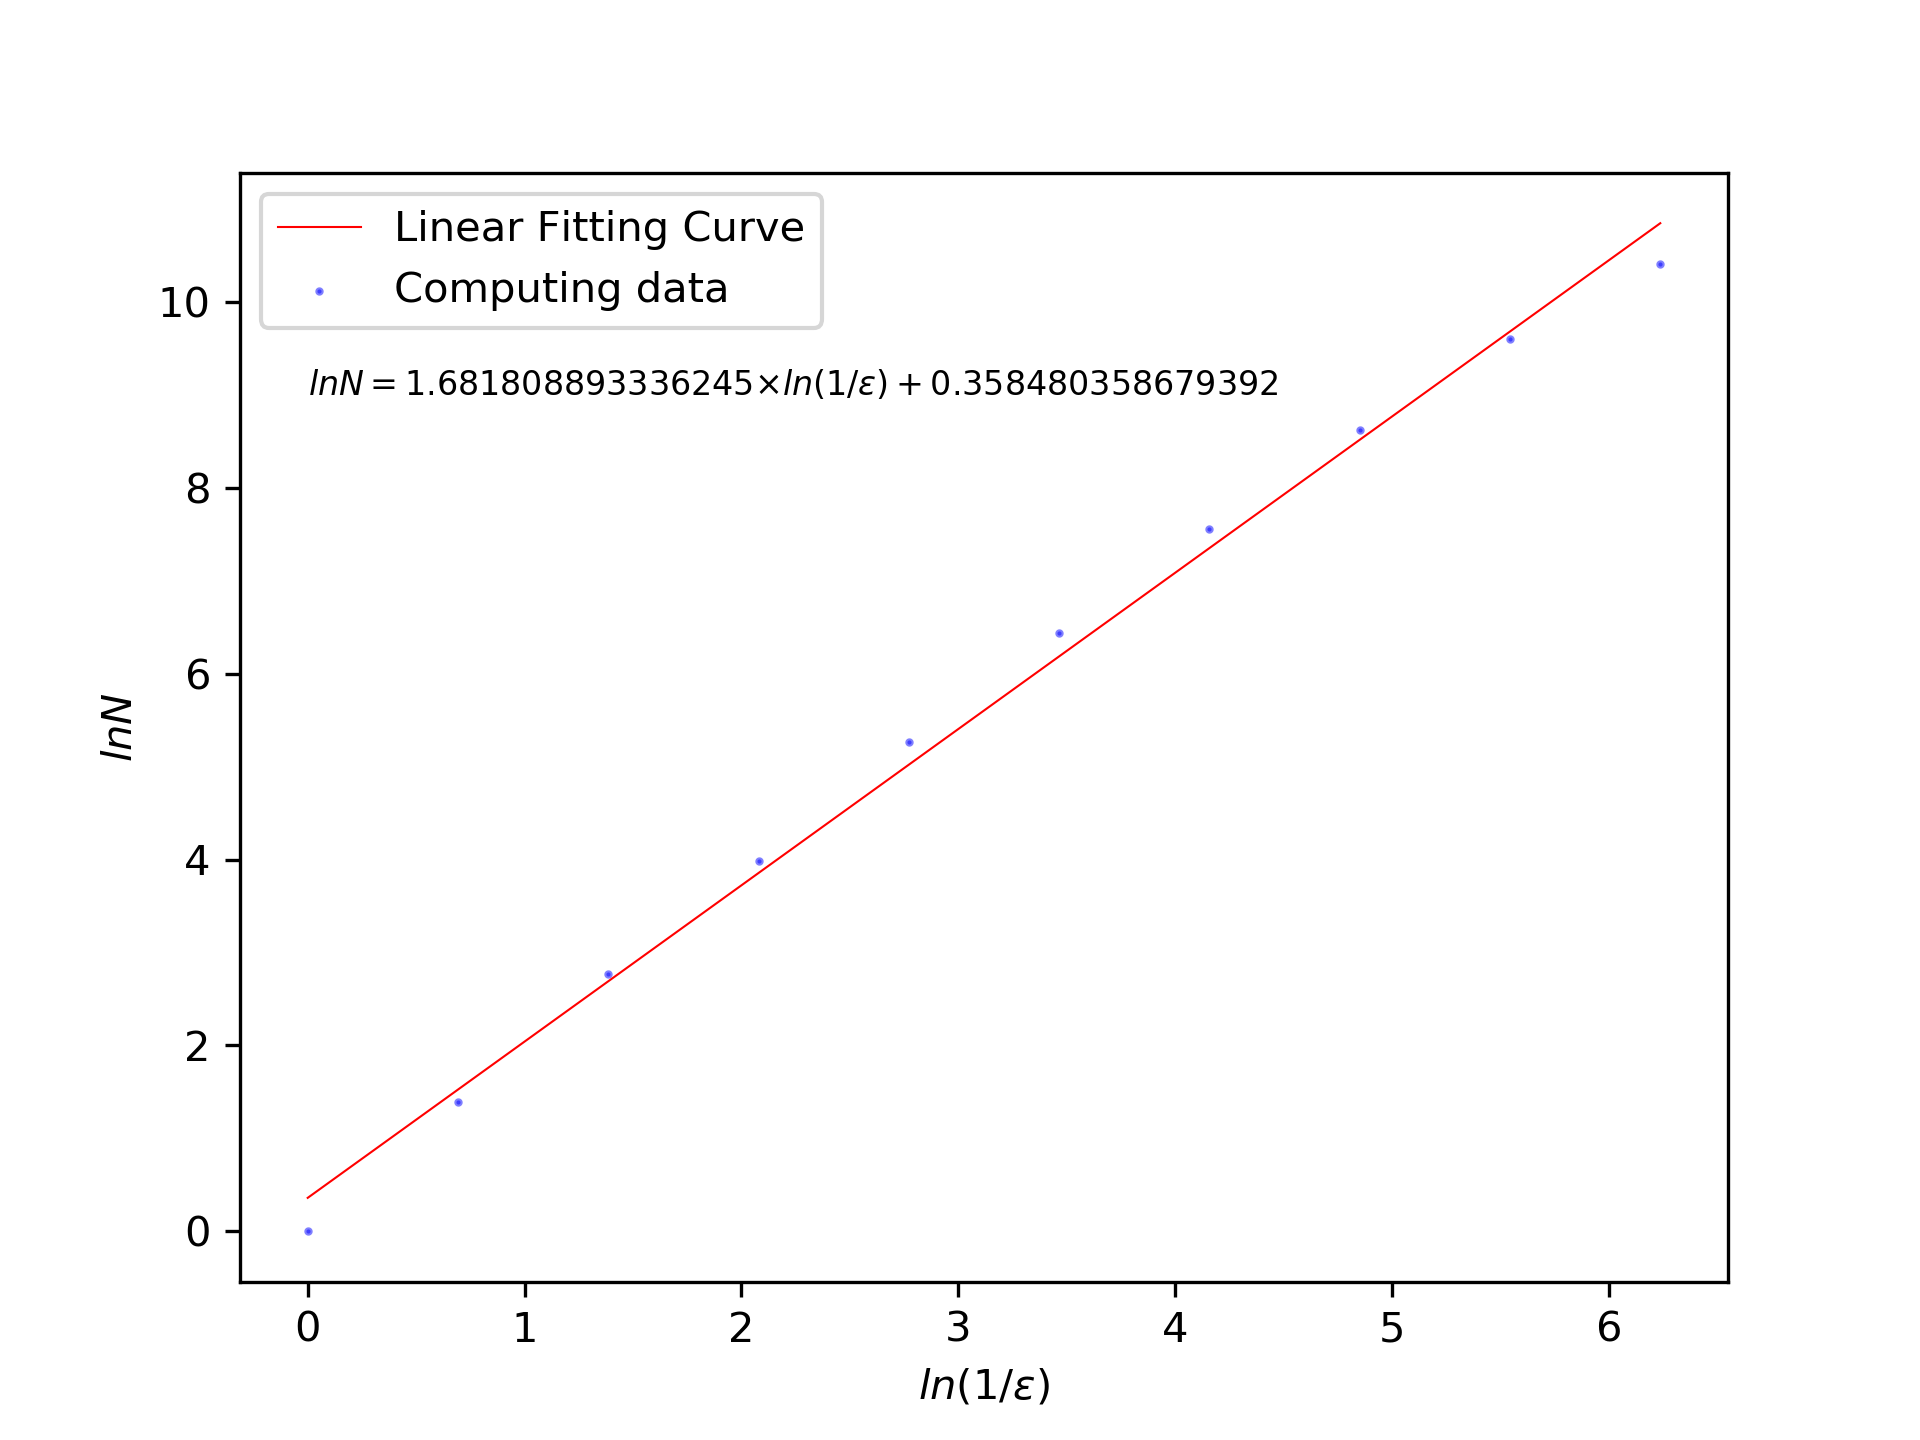
\includegraphics[bb= 0 0 460.8 345.6, width = 8cm]{分形维数/box-5-2*min-2.png}      
\caption{$R_{gen} = r_{cluster} + 5, R_{esp} = 2R_{gen}$删掉最后一个数据点的盒计数法}      
\end{figure}


\begin{figure}[!htbp]        
\centering
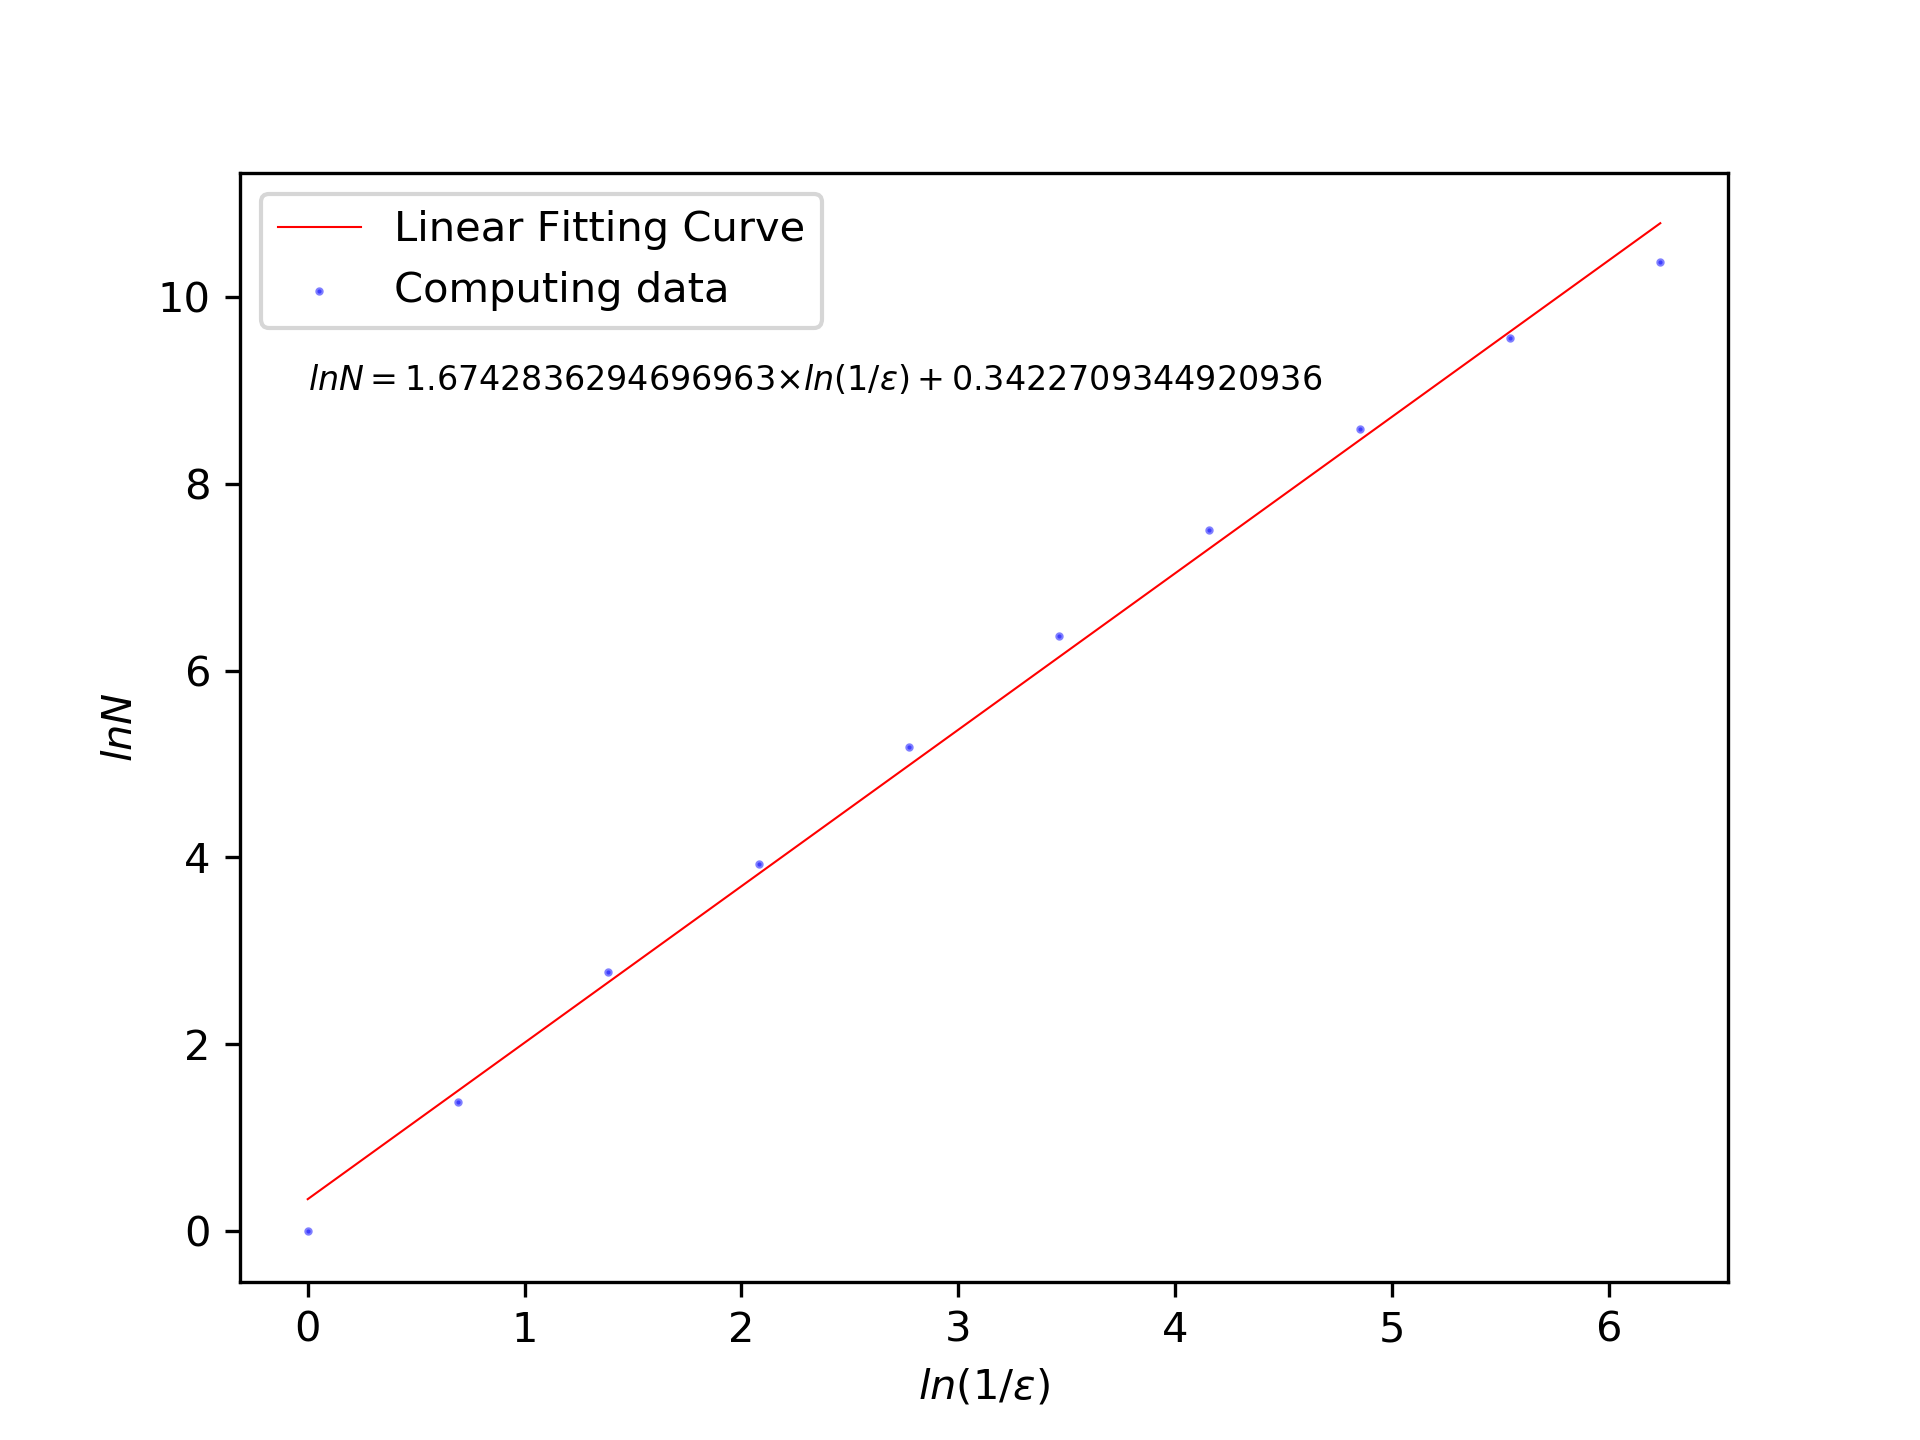
\includegraphics[bb= 0 0 460.8 345.6, width = 8cm]{分形维数/box-5-2.5*min-2.png}      
\caption{$R_{gen} = r_{cluster} + 5, R_{esp} = 2.5R_{gen}$删掉最后一个数据点的盒计数法}      
\end{figure}


\begin{figure}[!htbp]        
\centering
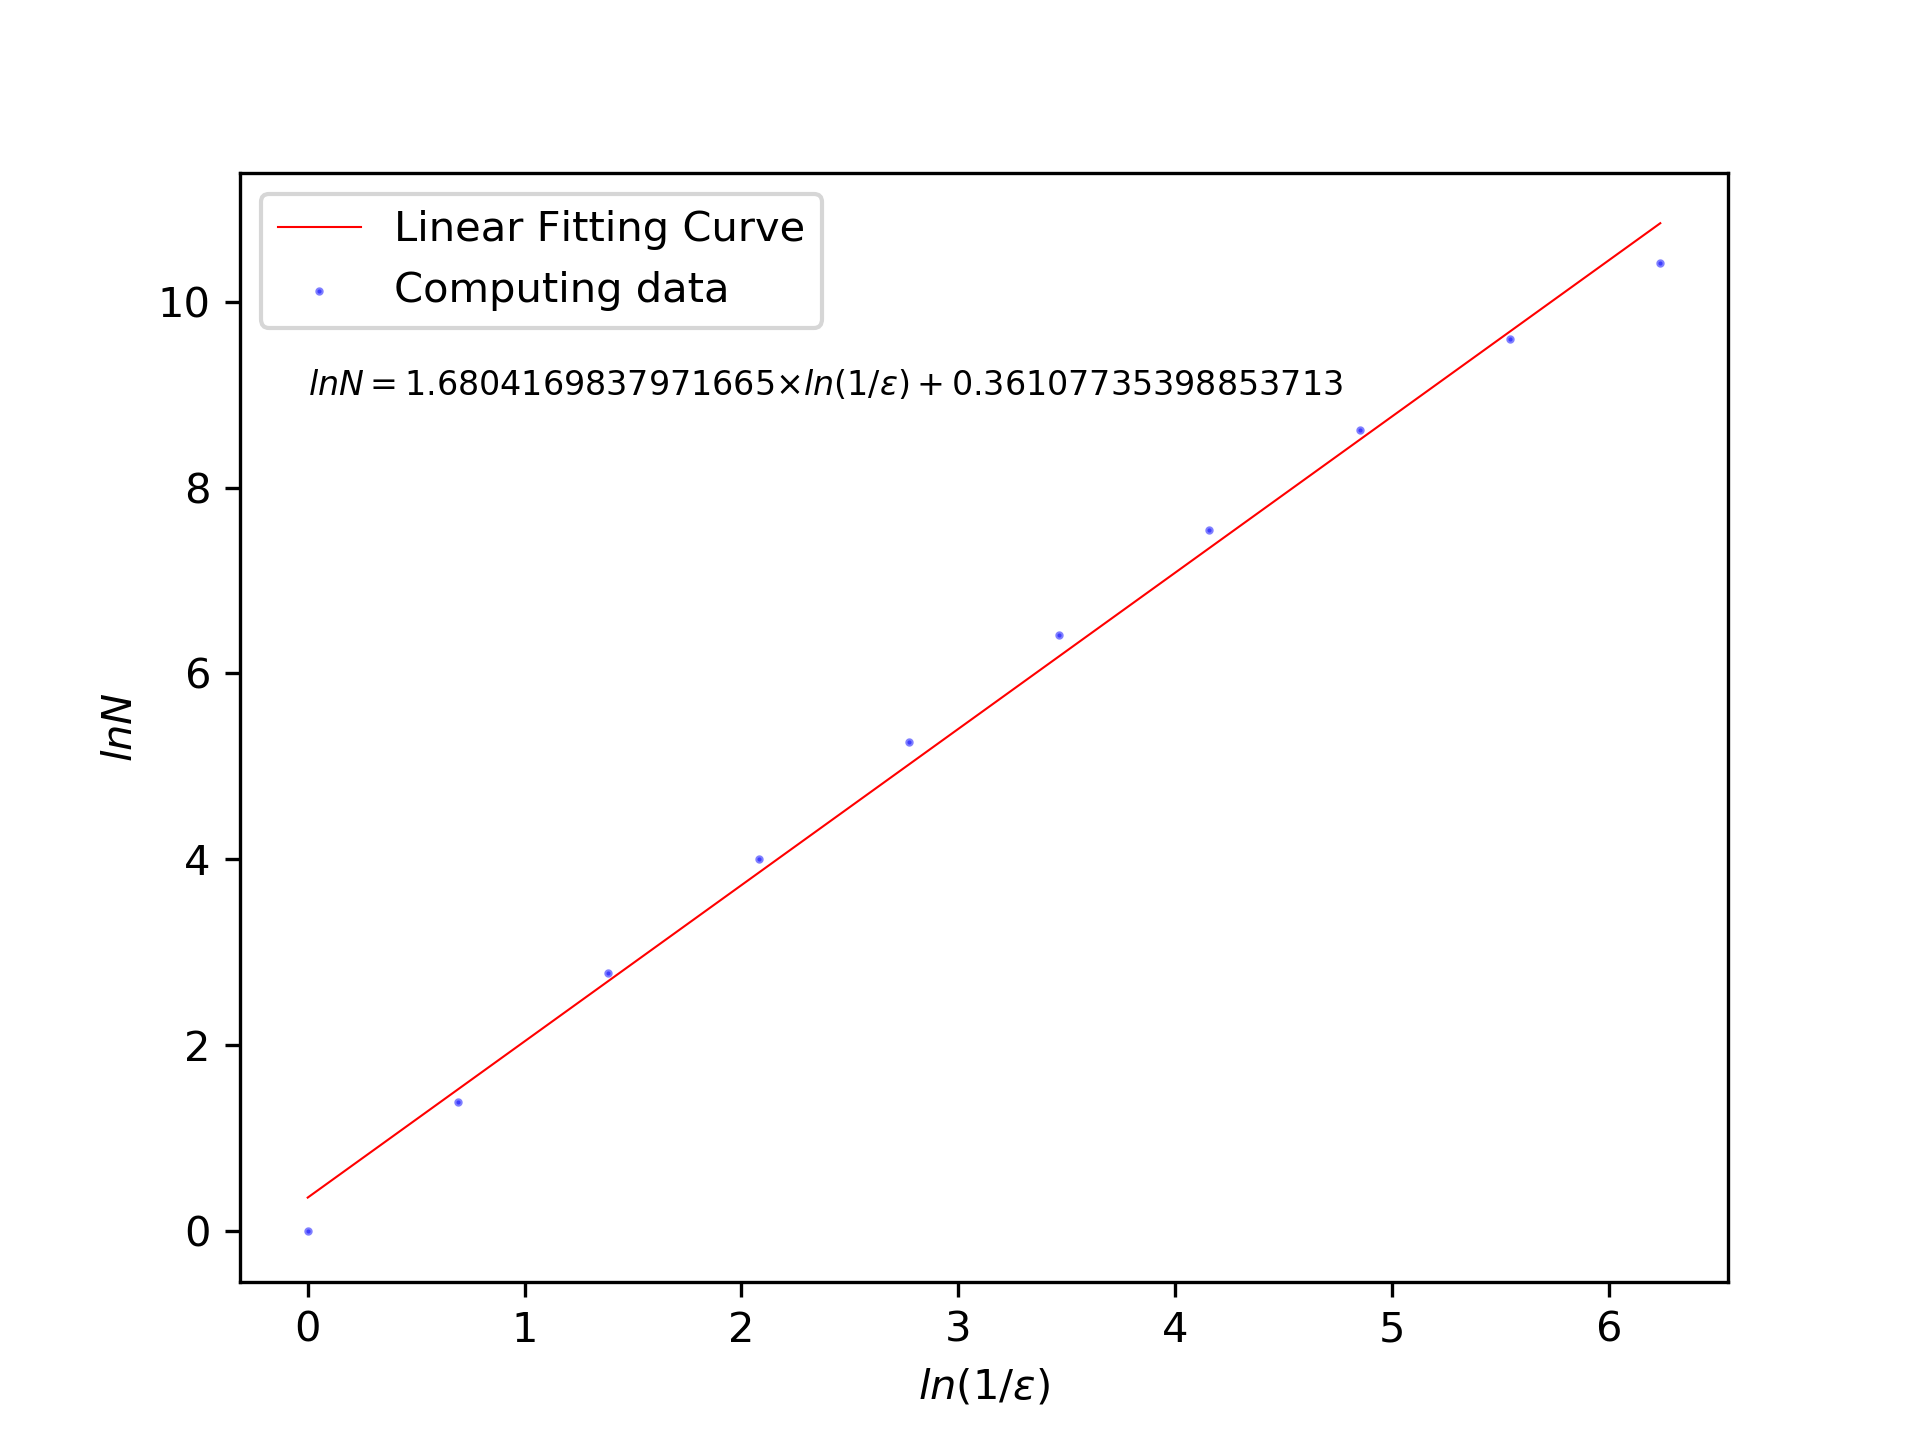
\includegraphics[bb= 0 0 460.8 345.6, width = 8cm]{分形维数/box-5-3*min-2.png}      
\caption{$R_{gen} = r_{cluster} + 5, R_{esp} = 3R_{gen}$删掉最后一个数据点的盒计数法}      
\end{figure}

\newpage
可以看出删掉最后一个数据点后,盒计数法得到的分形维数与Sandbox法得出的结果相差不大。具体原因目前并不清楚。



\subsection{有趣的讨论——逃逸区域对于结果的影响}

由于在实际情况下,某粒子可以随机行走到很远的地方(例如电解很稀的$CuSO_{4}$溶液时,容器边界相对于团簇大小来说很远),故逃逸边界只是数值模拟所必须的条件,且设置成为可动的边界是为了提高程序的运行速度。根据计算物理讲义上写到的一般取粒子产生边界大于团簇边界5个单位,逃逸边界设置为产生边界的$2\sim 3$倍。

\begin{figure}[!htbp]        
\centering
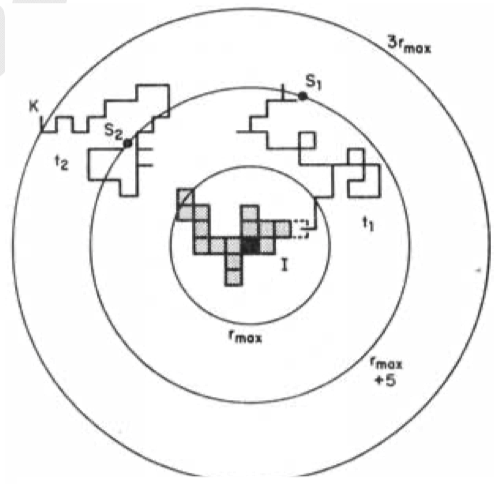
\includegraphics[ width = 4cm]{example.png}      
\caption{计算物理讲义上的DLA算法边界半径设置示意图}      
\end{figure}

故假设我们将逃逸半径的值设置的比较小时,看看结果会如何,有:

\begin{figure}[!htbp]        
\centering
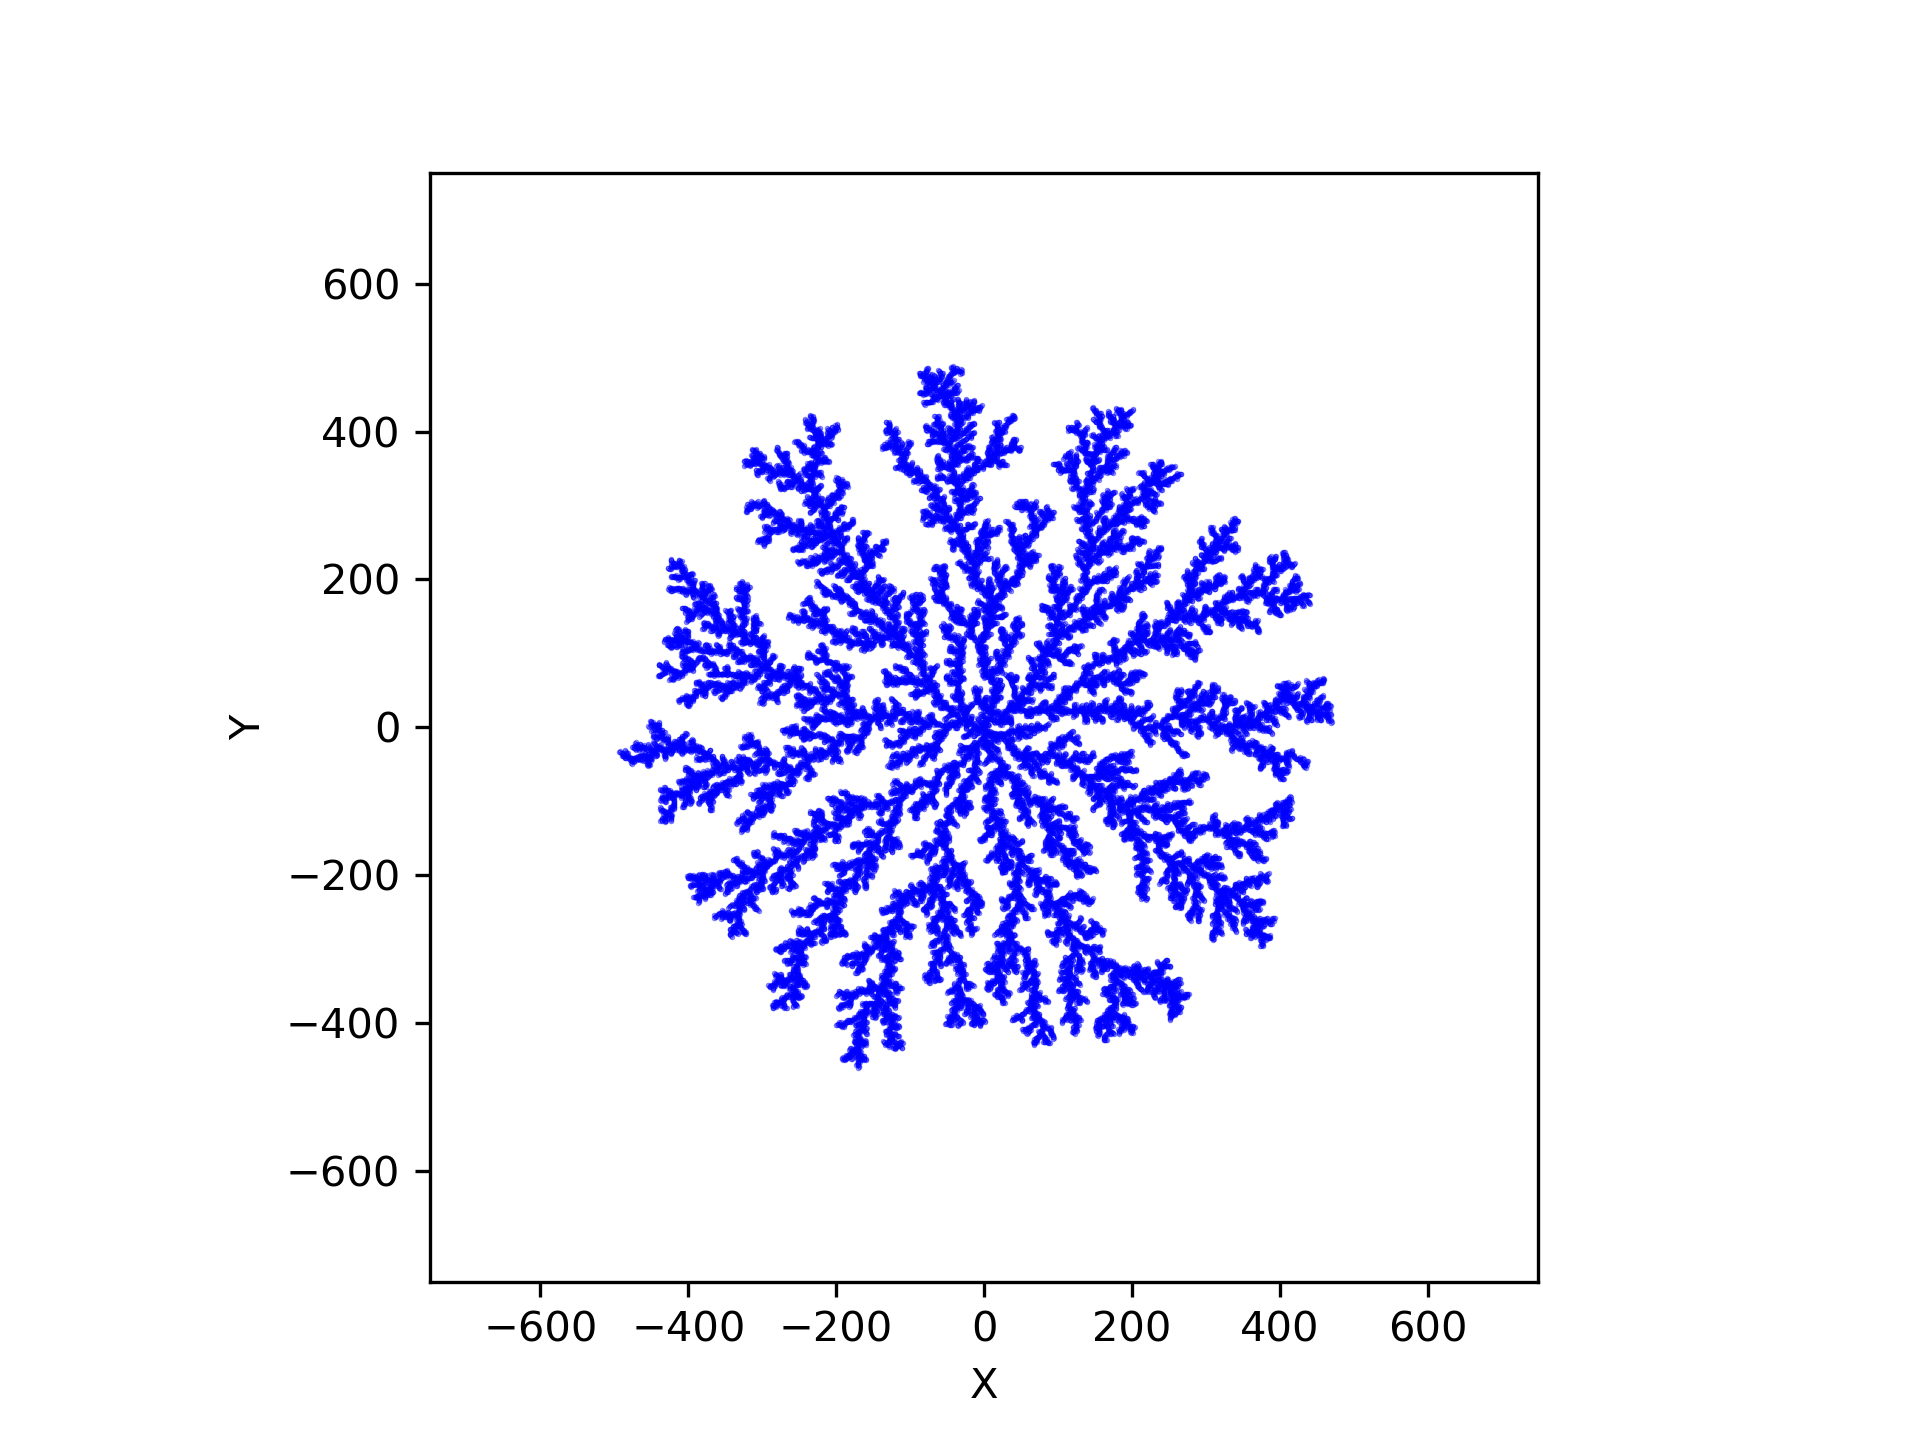
\includegraphics[bb= 0 0 460.8 345.6, width = 10cm]{改变max/1500-5*104-5-1.1*min.png}      
\caption{$R_{gen} = r_{cluster} + 5, R_{esp} = 1.1R_{gen}$的可视化模拟结果}      
\end{figure}


\begin{figure}[!htbp]        
\centering
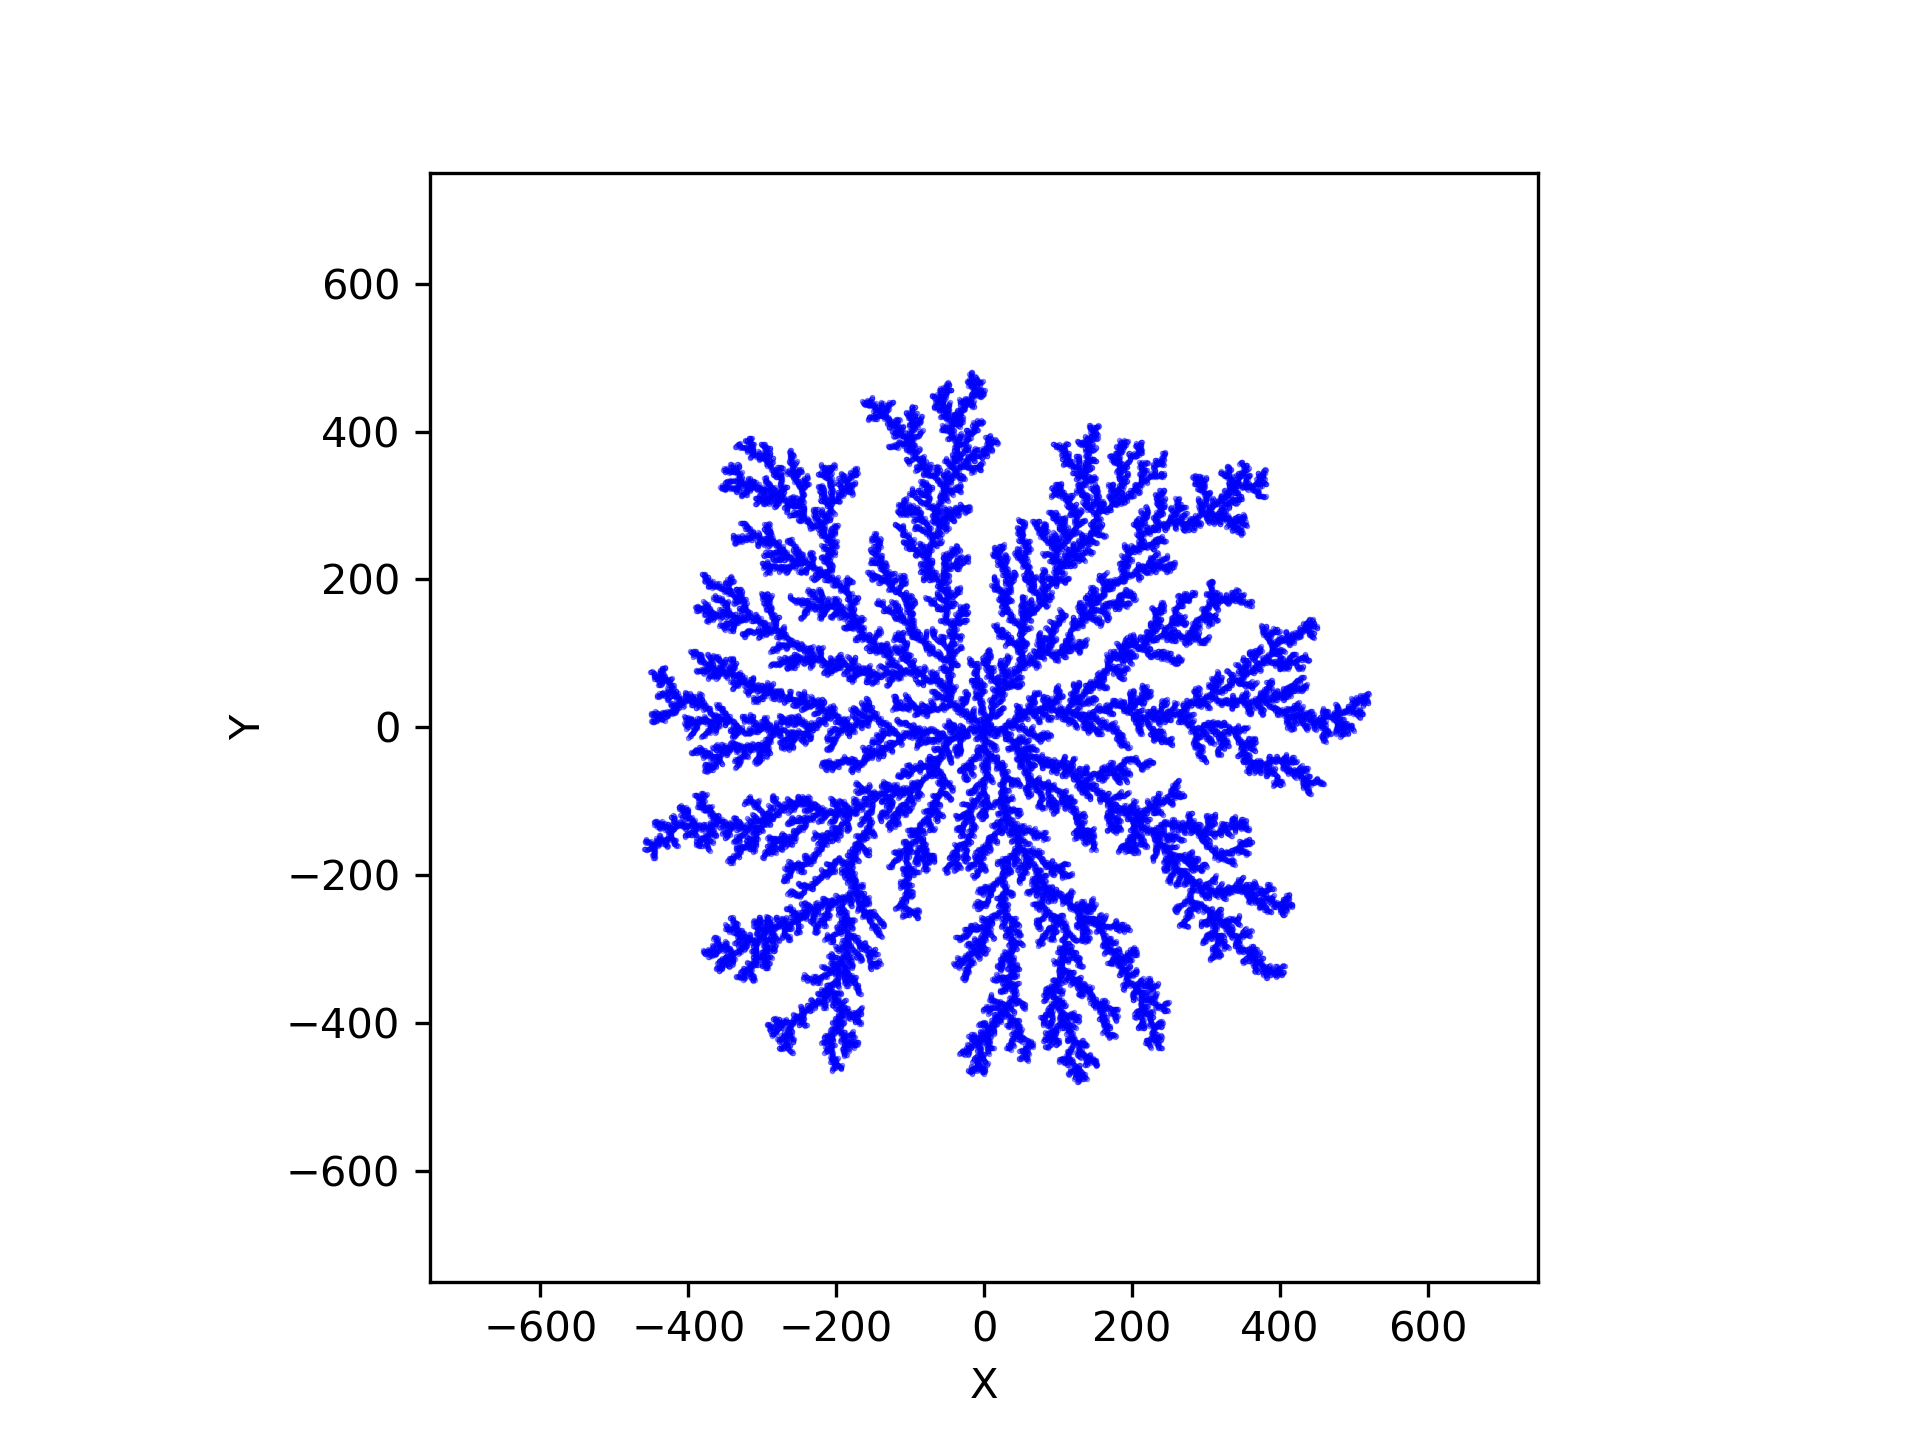
\includegraphics[bb= 0 0 460.8 345.6, width = 10cm]{改变max/1500-5*104-5-1.5*min.png}      
\caption{$R_{gen} = r_{cluster} + 5, R_{esp} = 1.5R_{gen}$的可视化模拟结果}      
\end{figure}


可以看到逃逸半径的减少,使DLA团簇更加密集。

\newpage 若这样变化的趋势不够明显,下面有更加夸张的结果,将逃逸半径的值改为产生半径的值加上某一定值\footnote{注意此处逃逸半径的设置并不是很科学,因为半径的设置应与团簇的相对大小有关,而加上某一定值会使得边界与团簇的相对大小不断变化。但此处这么设置是为了夸张的展示此现象},得到:


\begin{figure}[!htbp]        
\centering
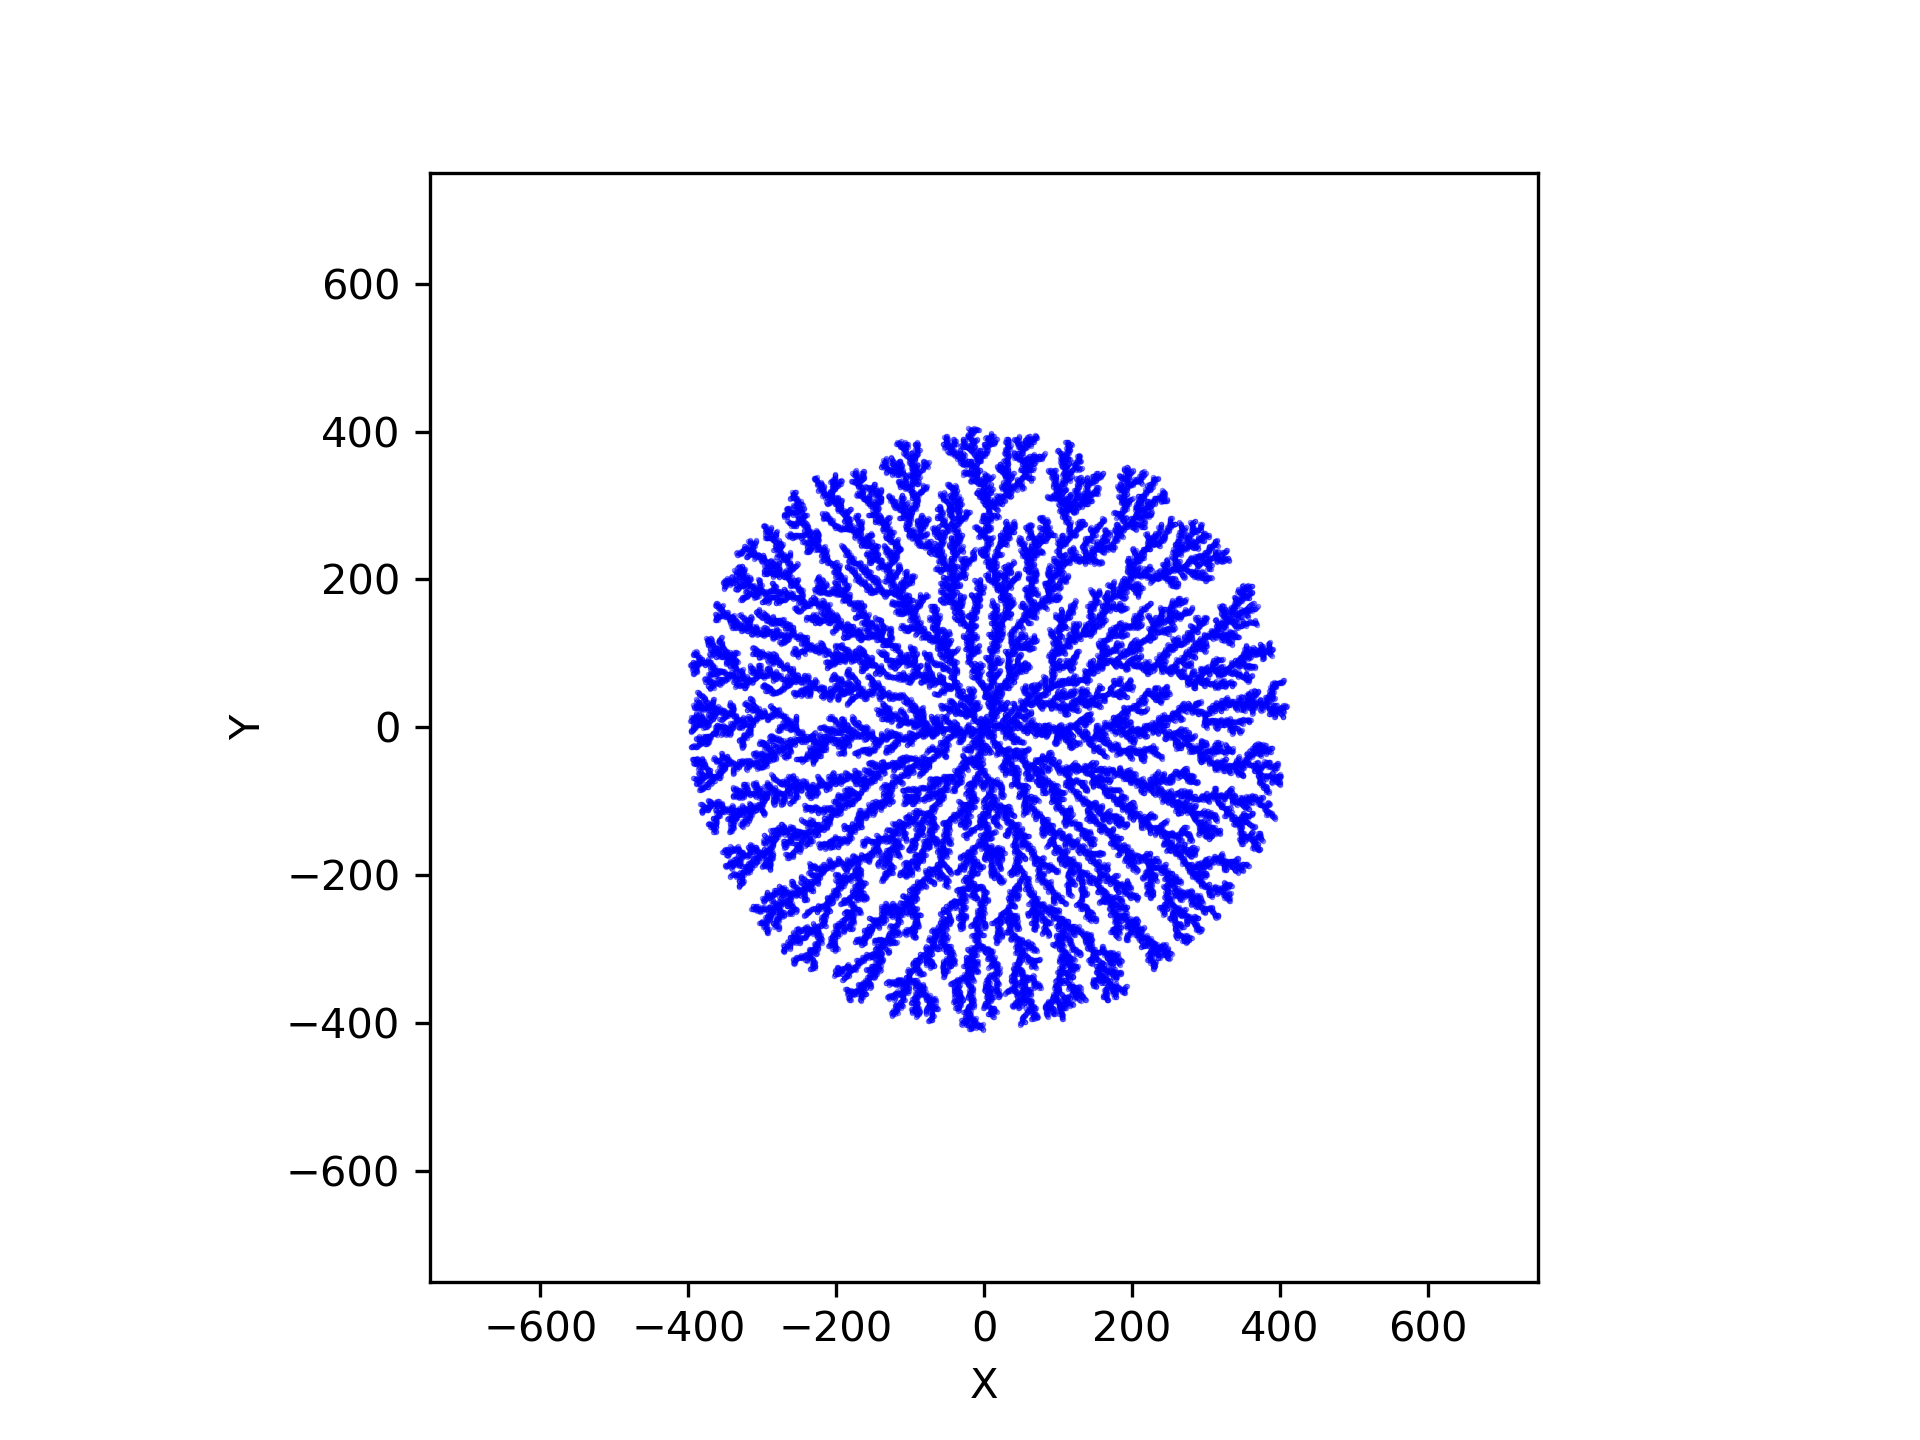
\includegraphics[bb= 0 0 460.8 345.6, width = 10cm]{改变max/5-7.png}      
\caption{$R_{gen} = r_{cluster} + 5, R_{esp} = R_{gen} + 2$的可视化模拟结果}      
\end{figure}


\begin{figure}[!htbp]        
\centering
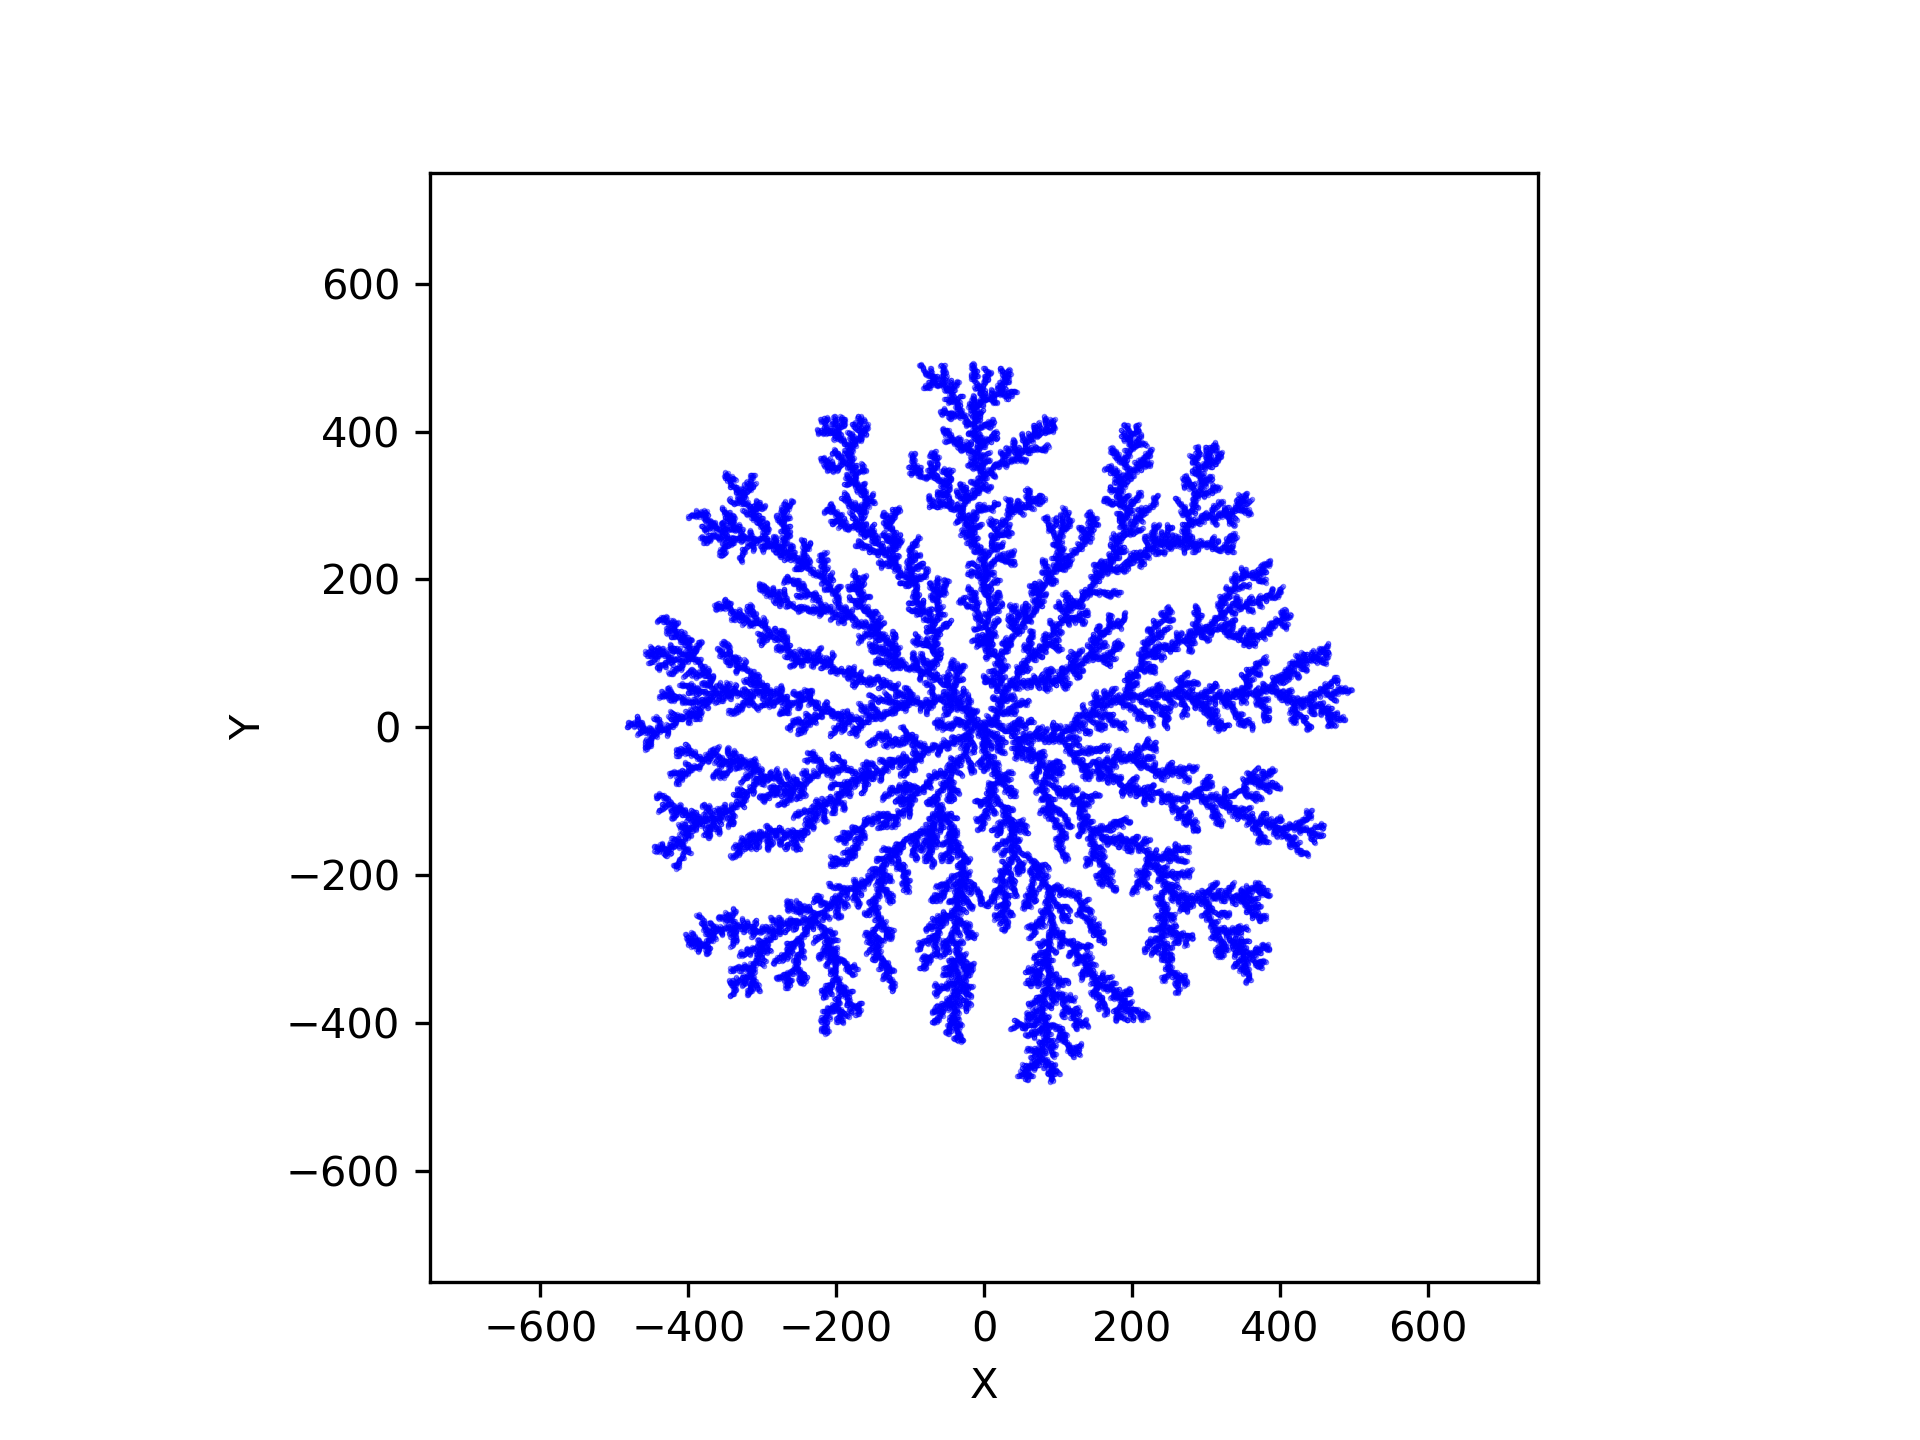
\includegraphics[bb= 0 0 460.8 345.6, width = 10cm]{改变max/5-55.png}      
\caption{$R_{gen} = r_{cluster} + 5, R_{esp} = R_{gen} + 50$的可视化模拟结果}      
\end{figure}


\begin{figure}[!htbp]        
\centering
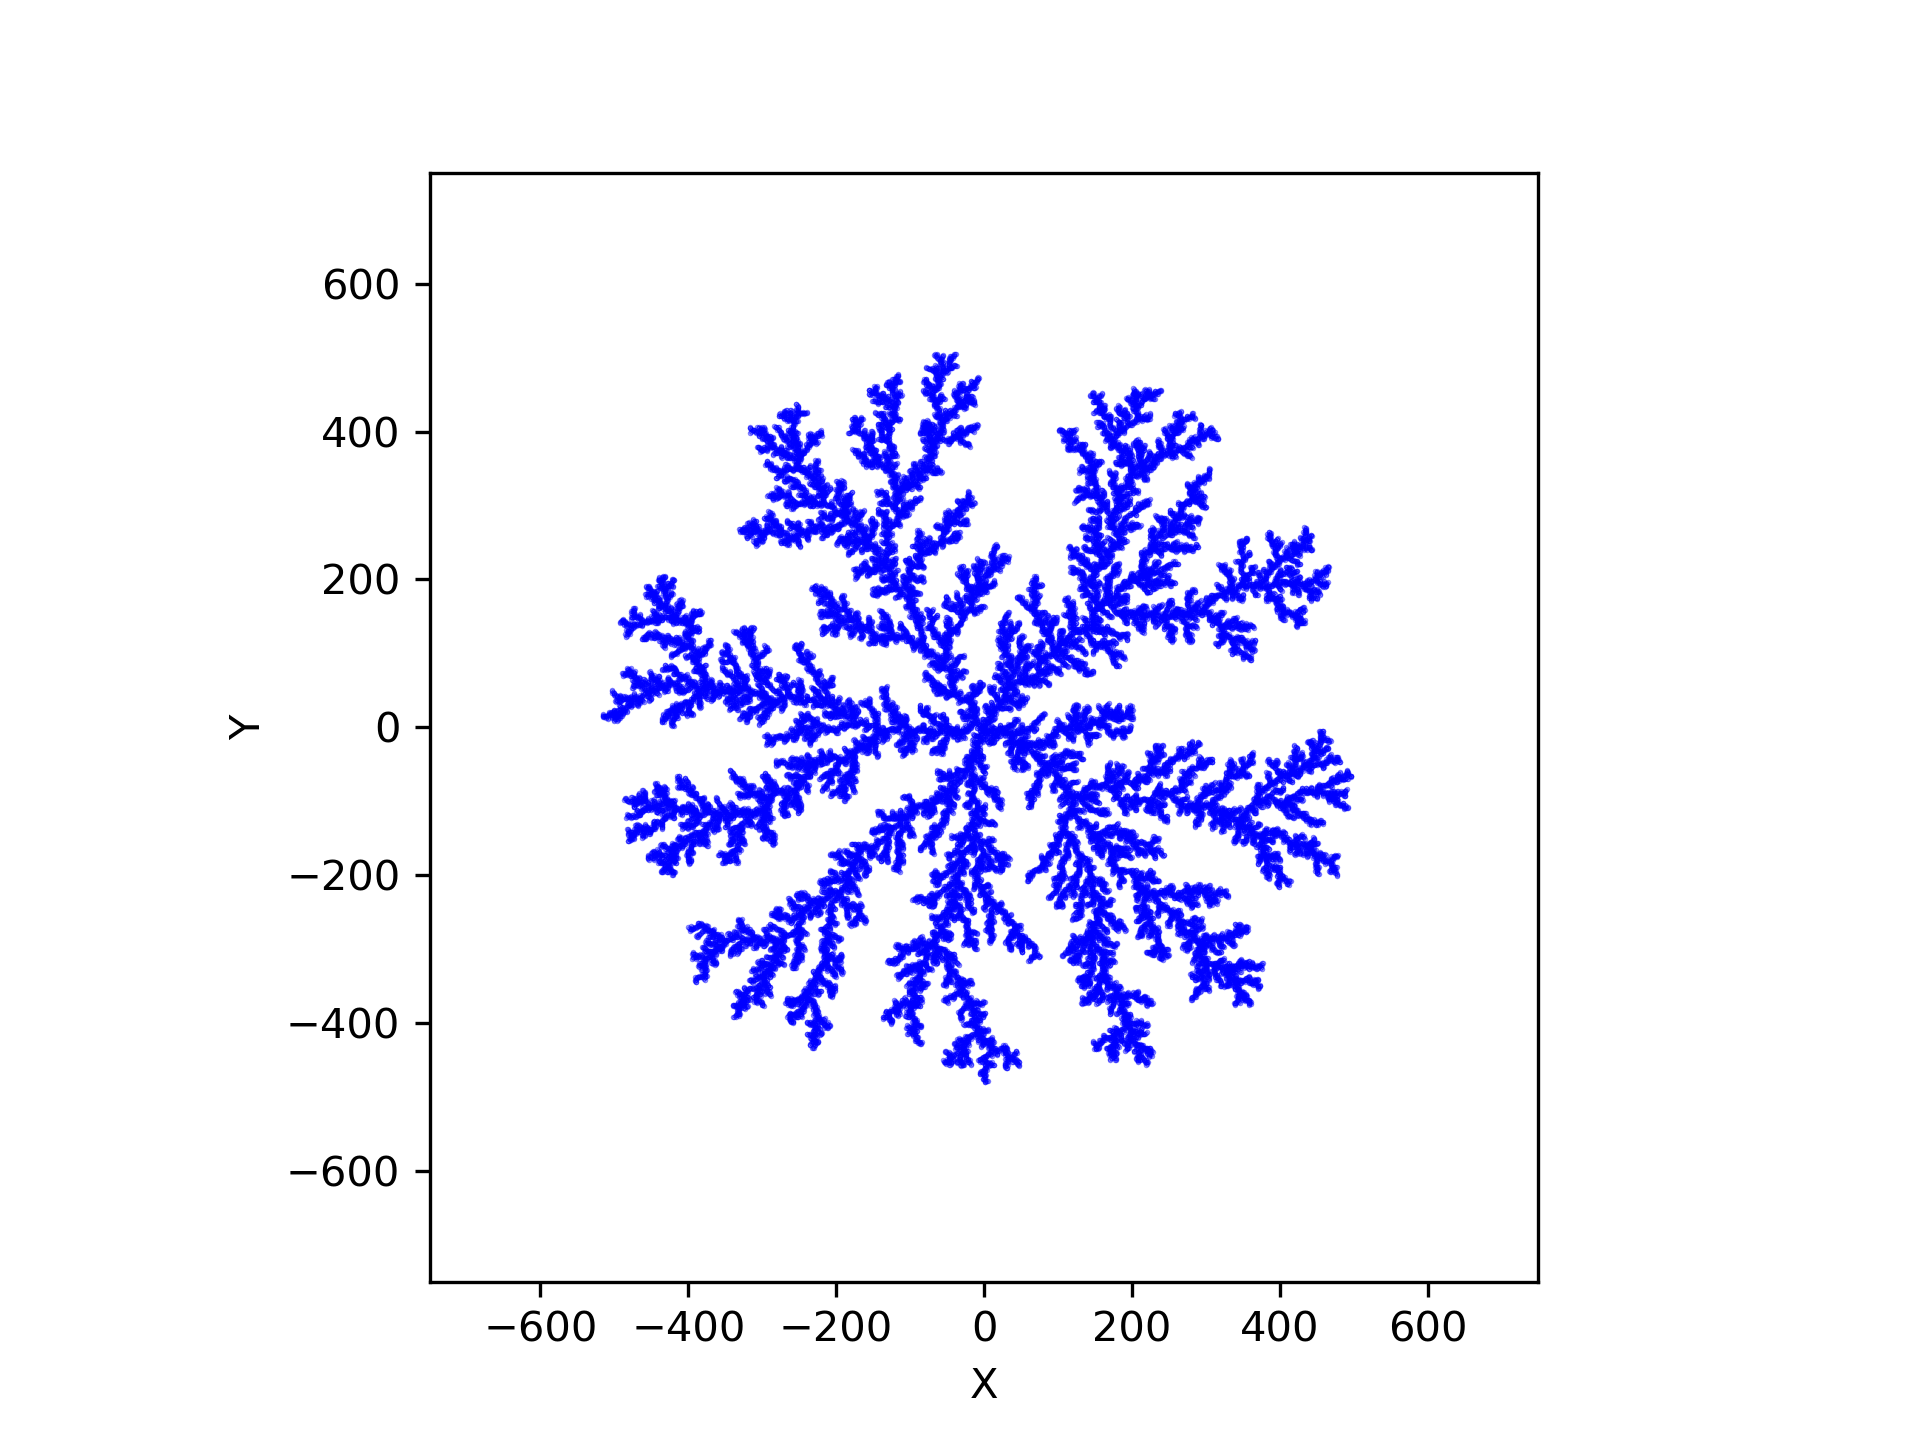
\includegraphics[bb= 0 0 460.8 345.6, width = 10cm]{改变max/5-205.png}      
\caption{$R_{gen} = r_{cluster} + 5, R_{esp} = R_{gen}+200$的可视化模拟结果}      
\end{figure}

\newpage 可以明显的看出此规律。为了定量描述此规律,我们对上面三种情况进行了分形维数的统计,得到:


\begin{figure}[!htbp]        
\centering
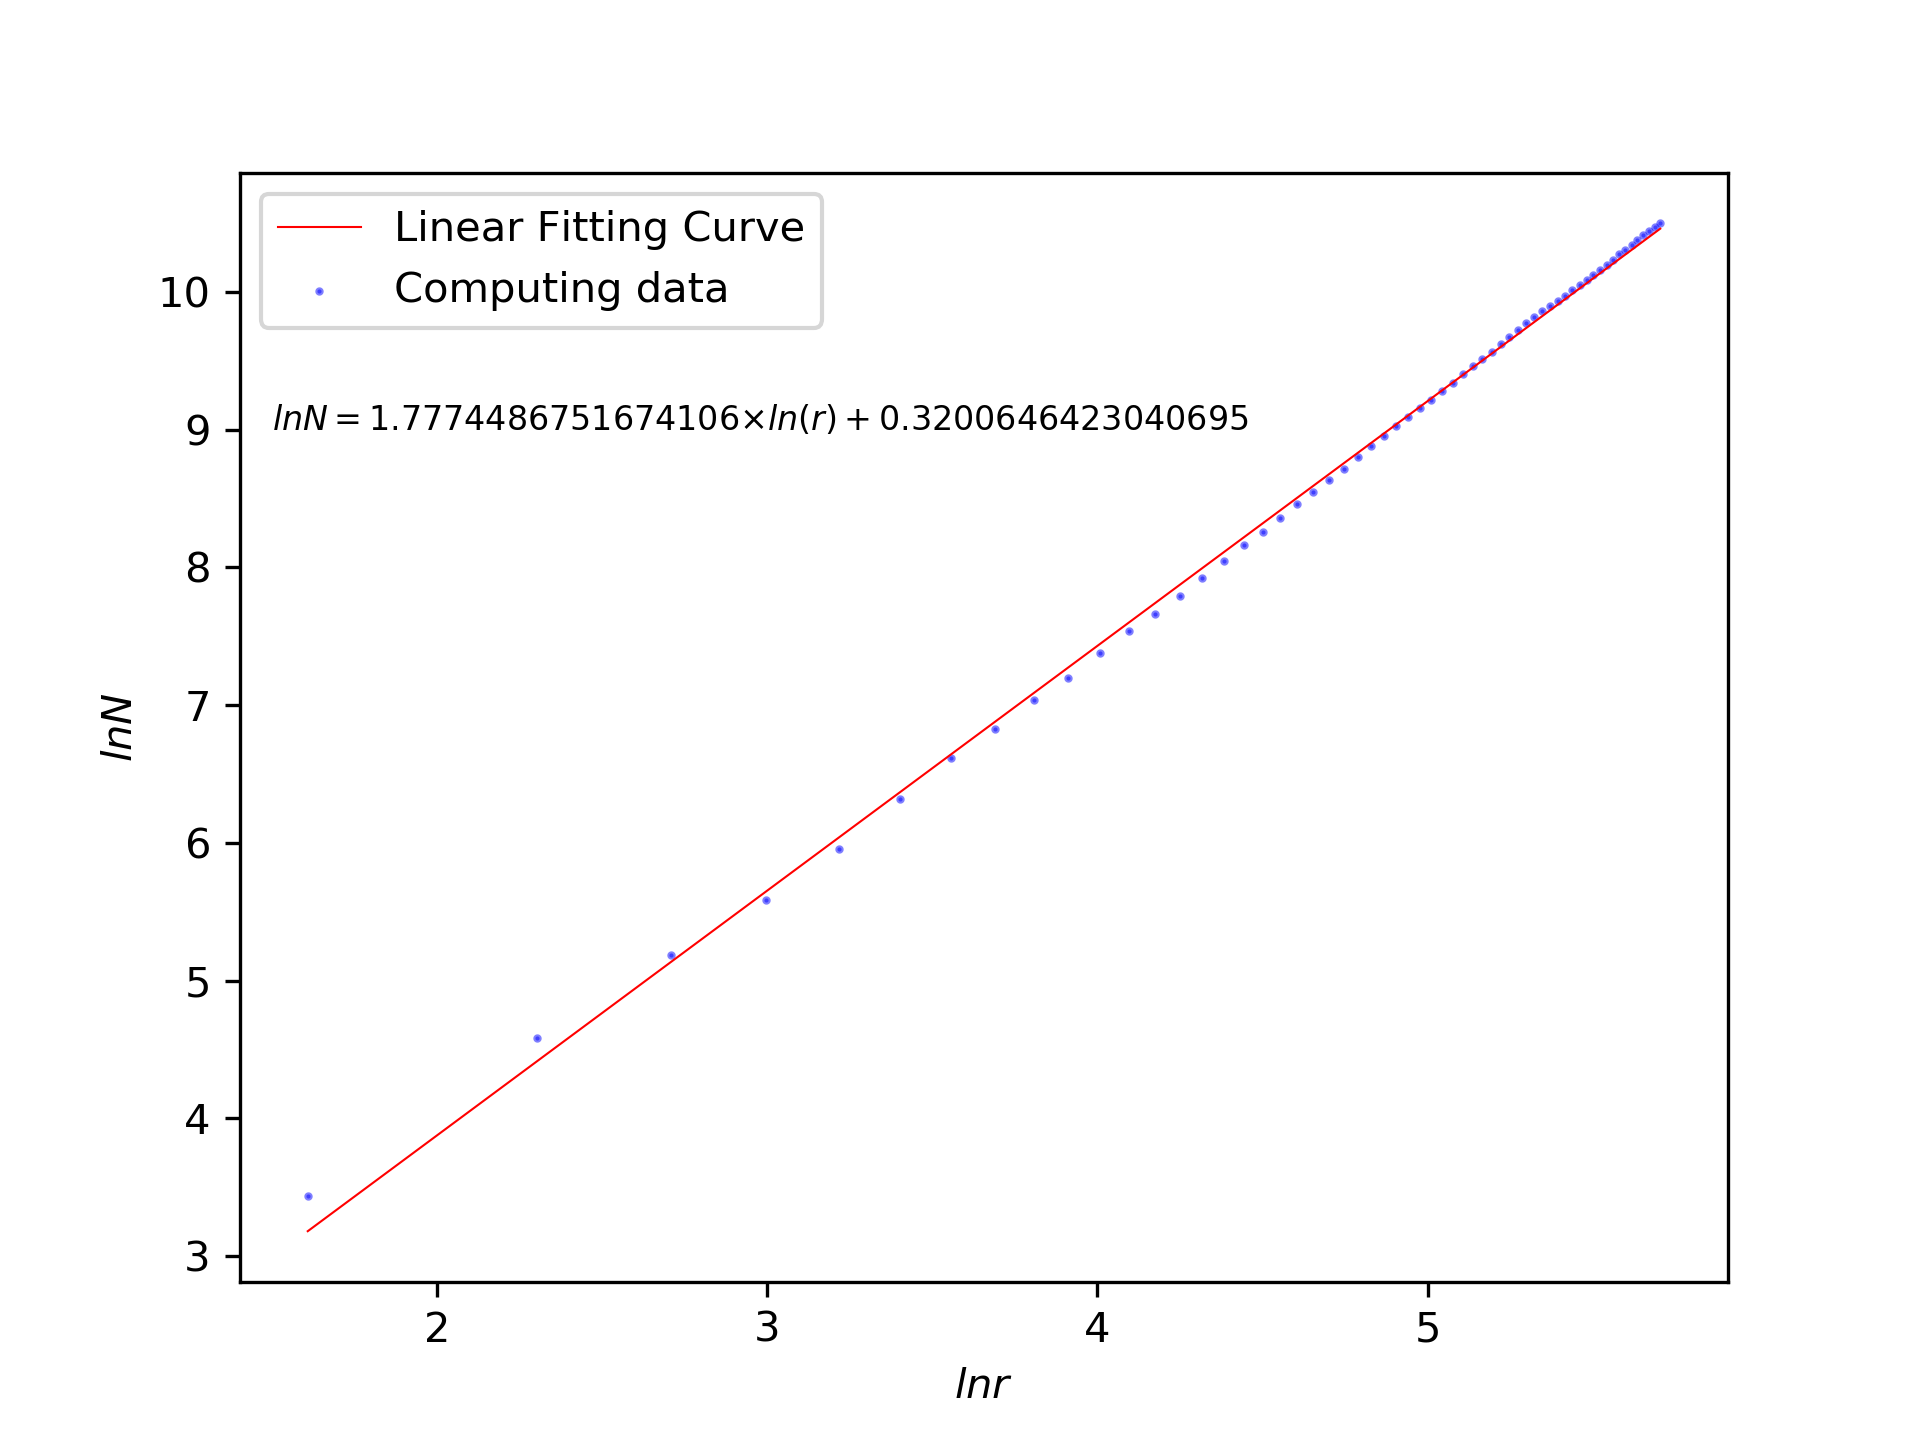
\includegraphics[bb= 0 0 460.8 345.6, width = 10cm]{分形维数/sandbox-5-7.png}      
\caption{$R_{gen} = r_{cluster} + 5, R_{esp} = R_{gen}+2$的Sandbox法计算分形维数}      
\end{figure}



\begin{figure}[!htbp]        
\centering
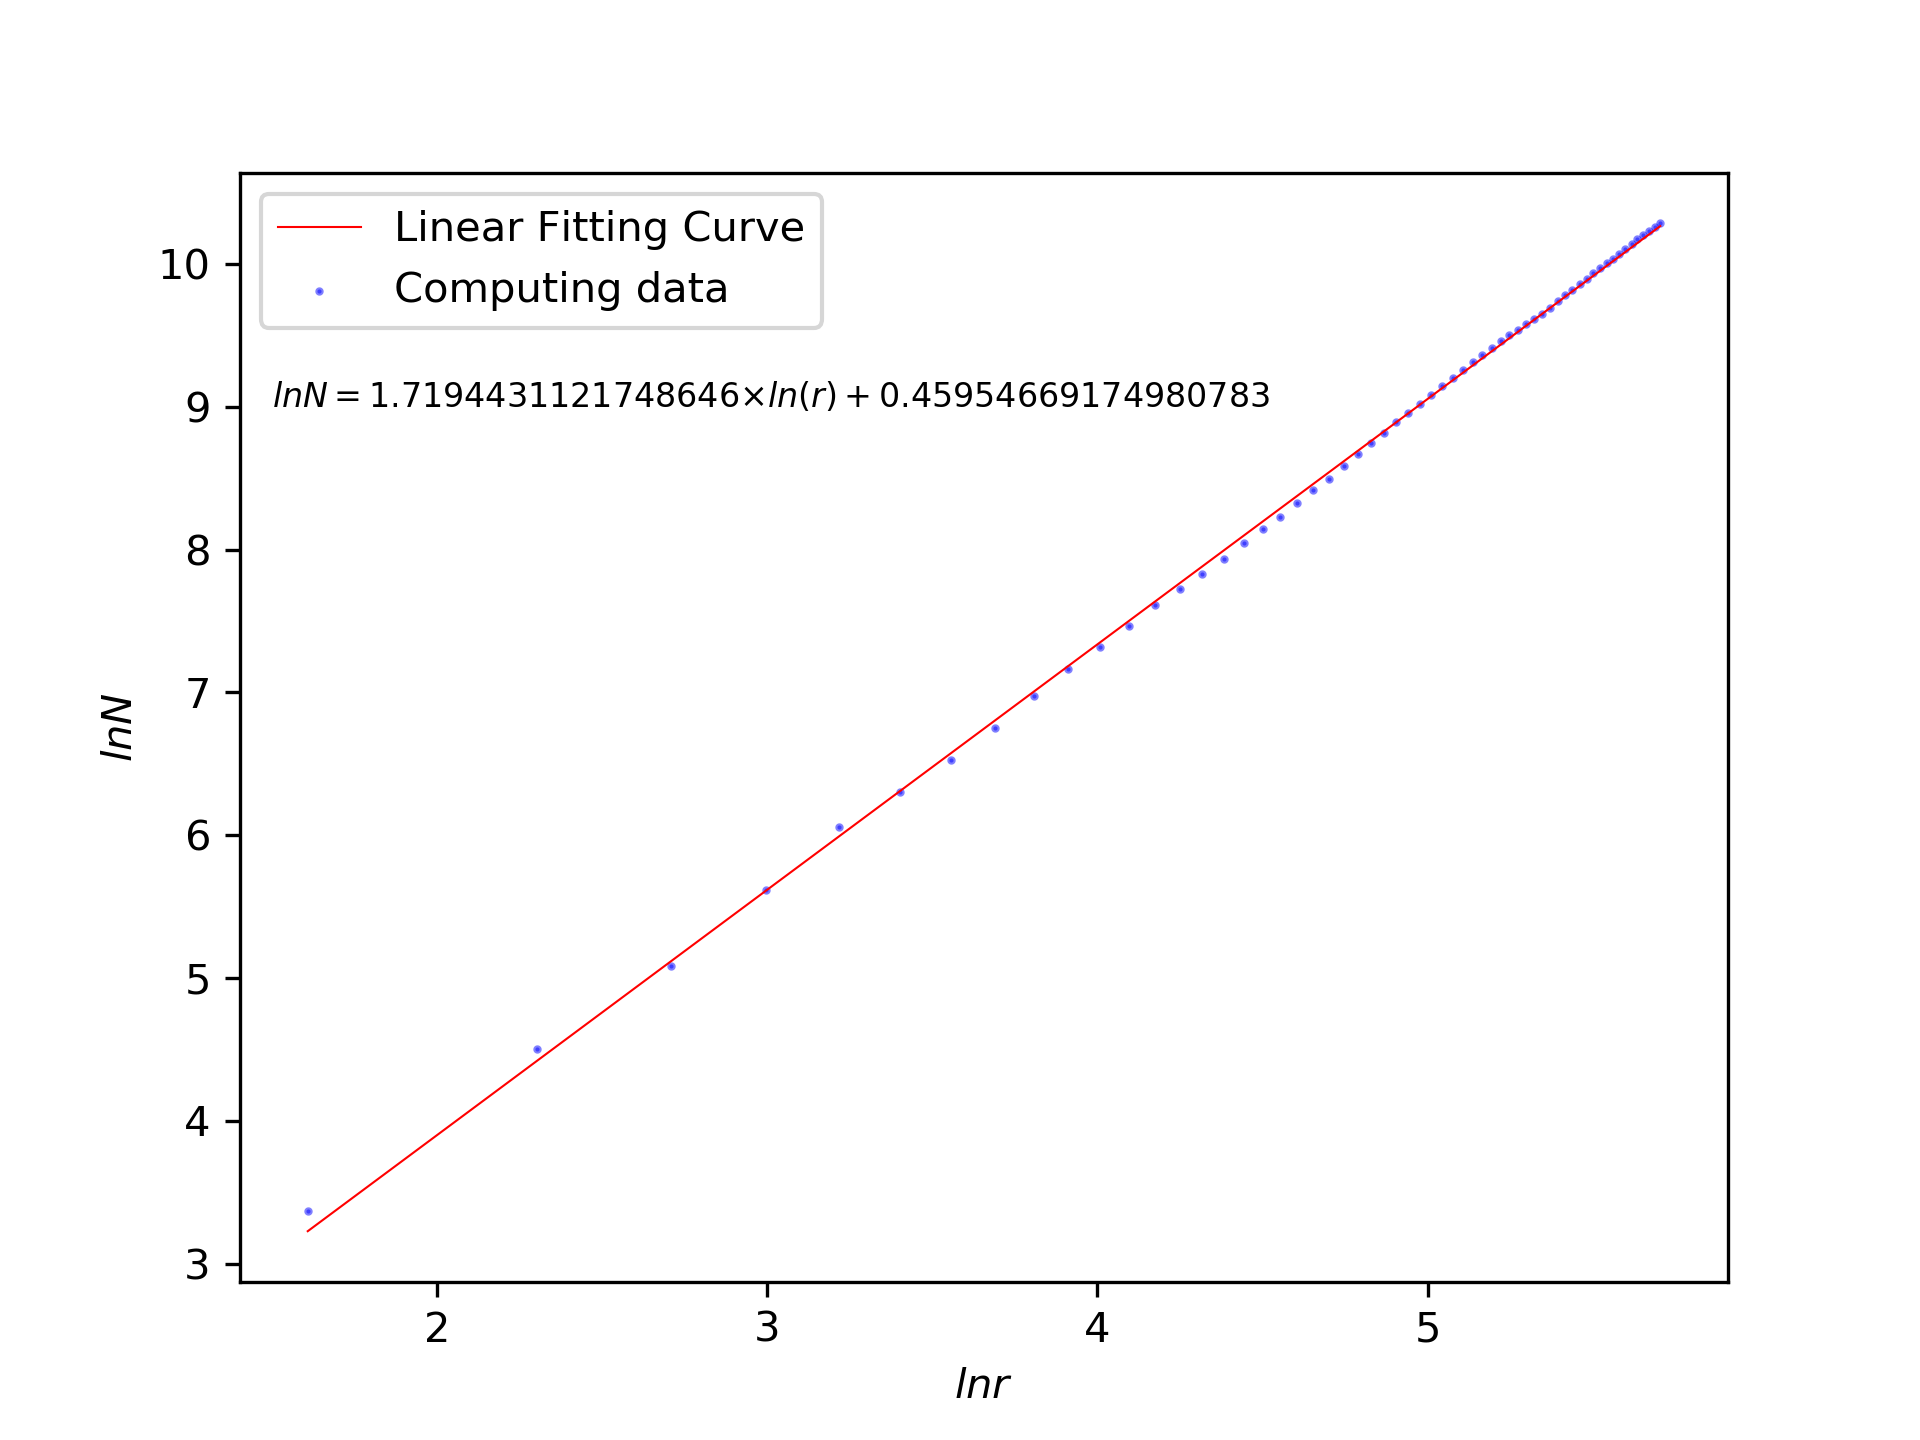
\includegraphics[bb= 0 0 460.8 345.6, width = 10cm]{分形维数/sandbox-5-55.png}      
\caption{$R_{gen} = r_{cluster} + 5, R_{esp} = R_{gen}+50$的Sandbox法计算分形维数}      
\end{figure}


\begin{figure}[!htbp]        
\centering
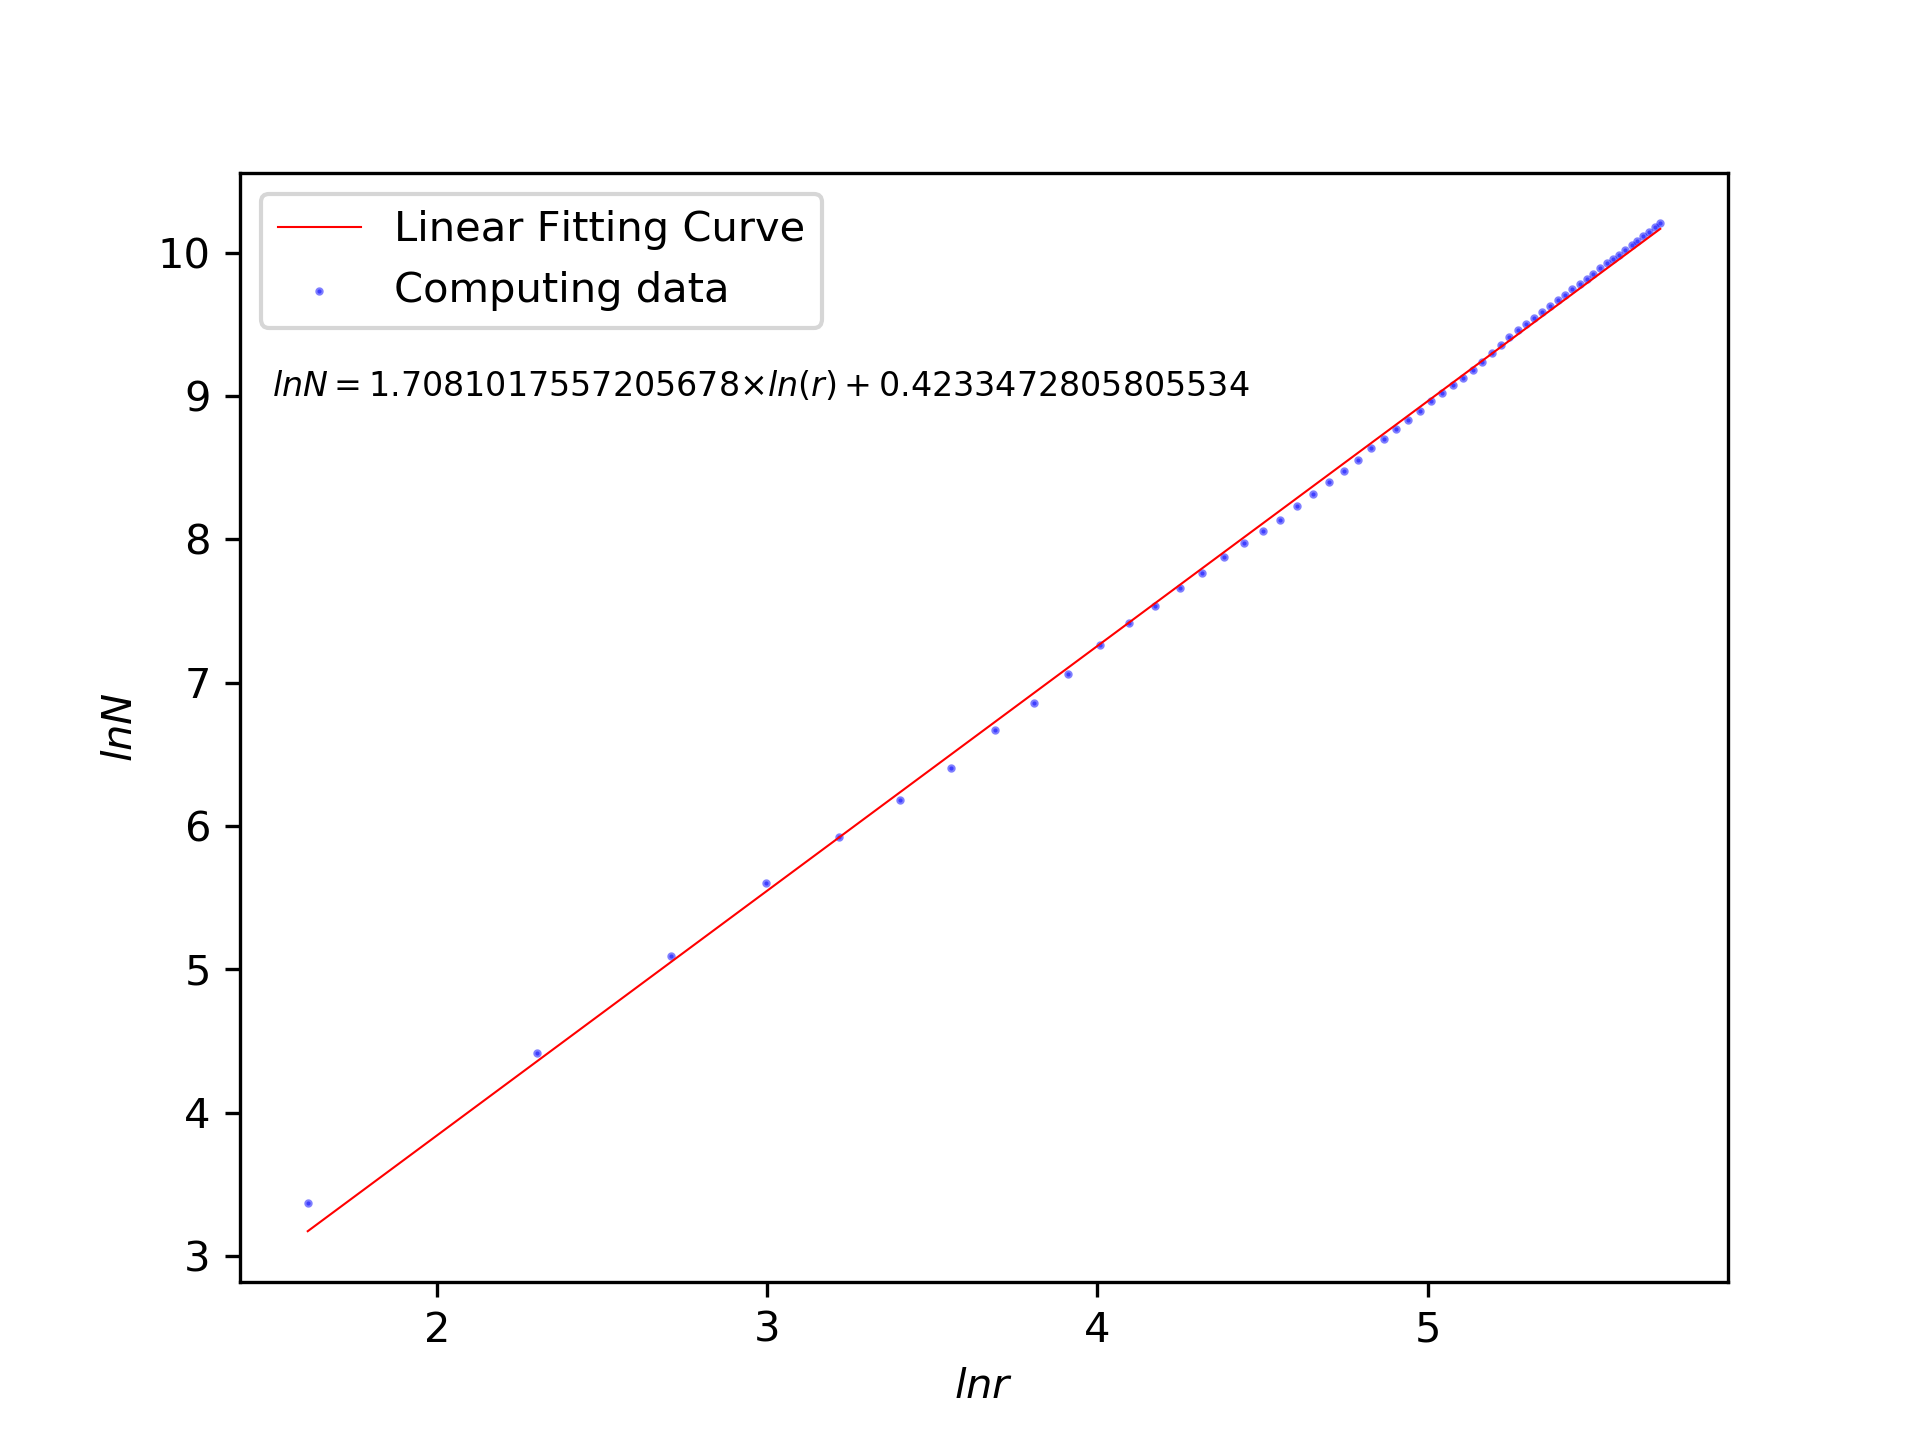
\includegraphics[bb= 0 0 460.8 345.6, width = 10cm]{分形维数/sandbox-5-205.png}      
\caption{$R_{gen} = r_{cluster} + 5, R_{esp} = R_{gen}+200$的Sandbox法计算分形维数}      
\end{figure}

\newpage
可以明显的看出随着逃逸半径的增大,分形维数越来越小,即图形越来越稀疏。

而产生这种现象的原因,个人认为实际团簇粒子生长过程或逃逸半径很大的时候,某随机粒子可游走到相对团簇粒子比较远的距离后并折返回来,到达与其实位置相差角度很大的地方(以团簇中心为原点,极坐标下的角度),从而有一部分随机粒子可以绕过在其实位置周围的团簇分支,到达别的地方。而若逃逸半径很小的时候,会导致这部分粒子几乎消失,从而粒子几乎只能到达在其实位置附近的团簇分支上。由于团簇的各项不均匀性会不断放大,故逃逸半径较小的模拟结果会使得团簇更加密集,此种现象应该与实际不符。故我们设置DLA模拟的逃逸半径时,应兼顾比较符合实际且计算量不会很大的值。


另外,本人一开始选取的边界为正方形边界,故导致模拟出来的团簇并不各项均匀:


\begin{figure}[!htbp]        
\centering
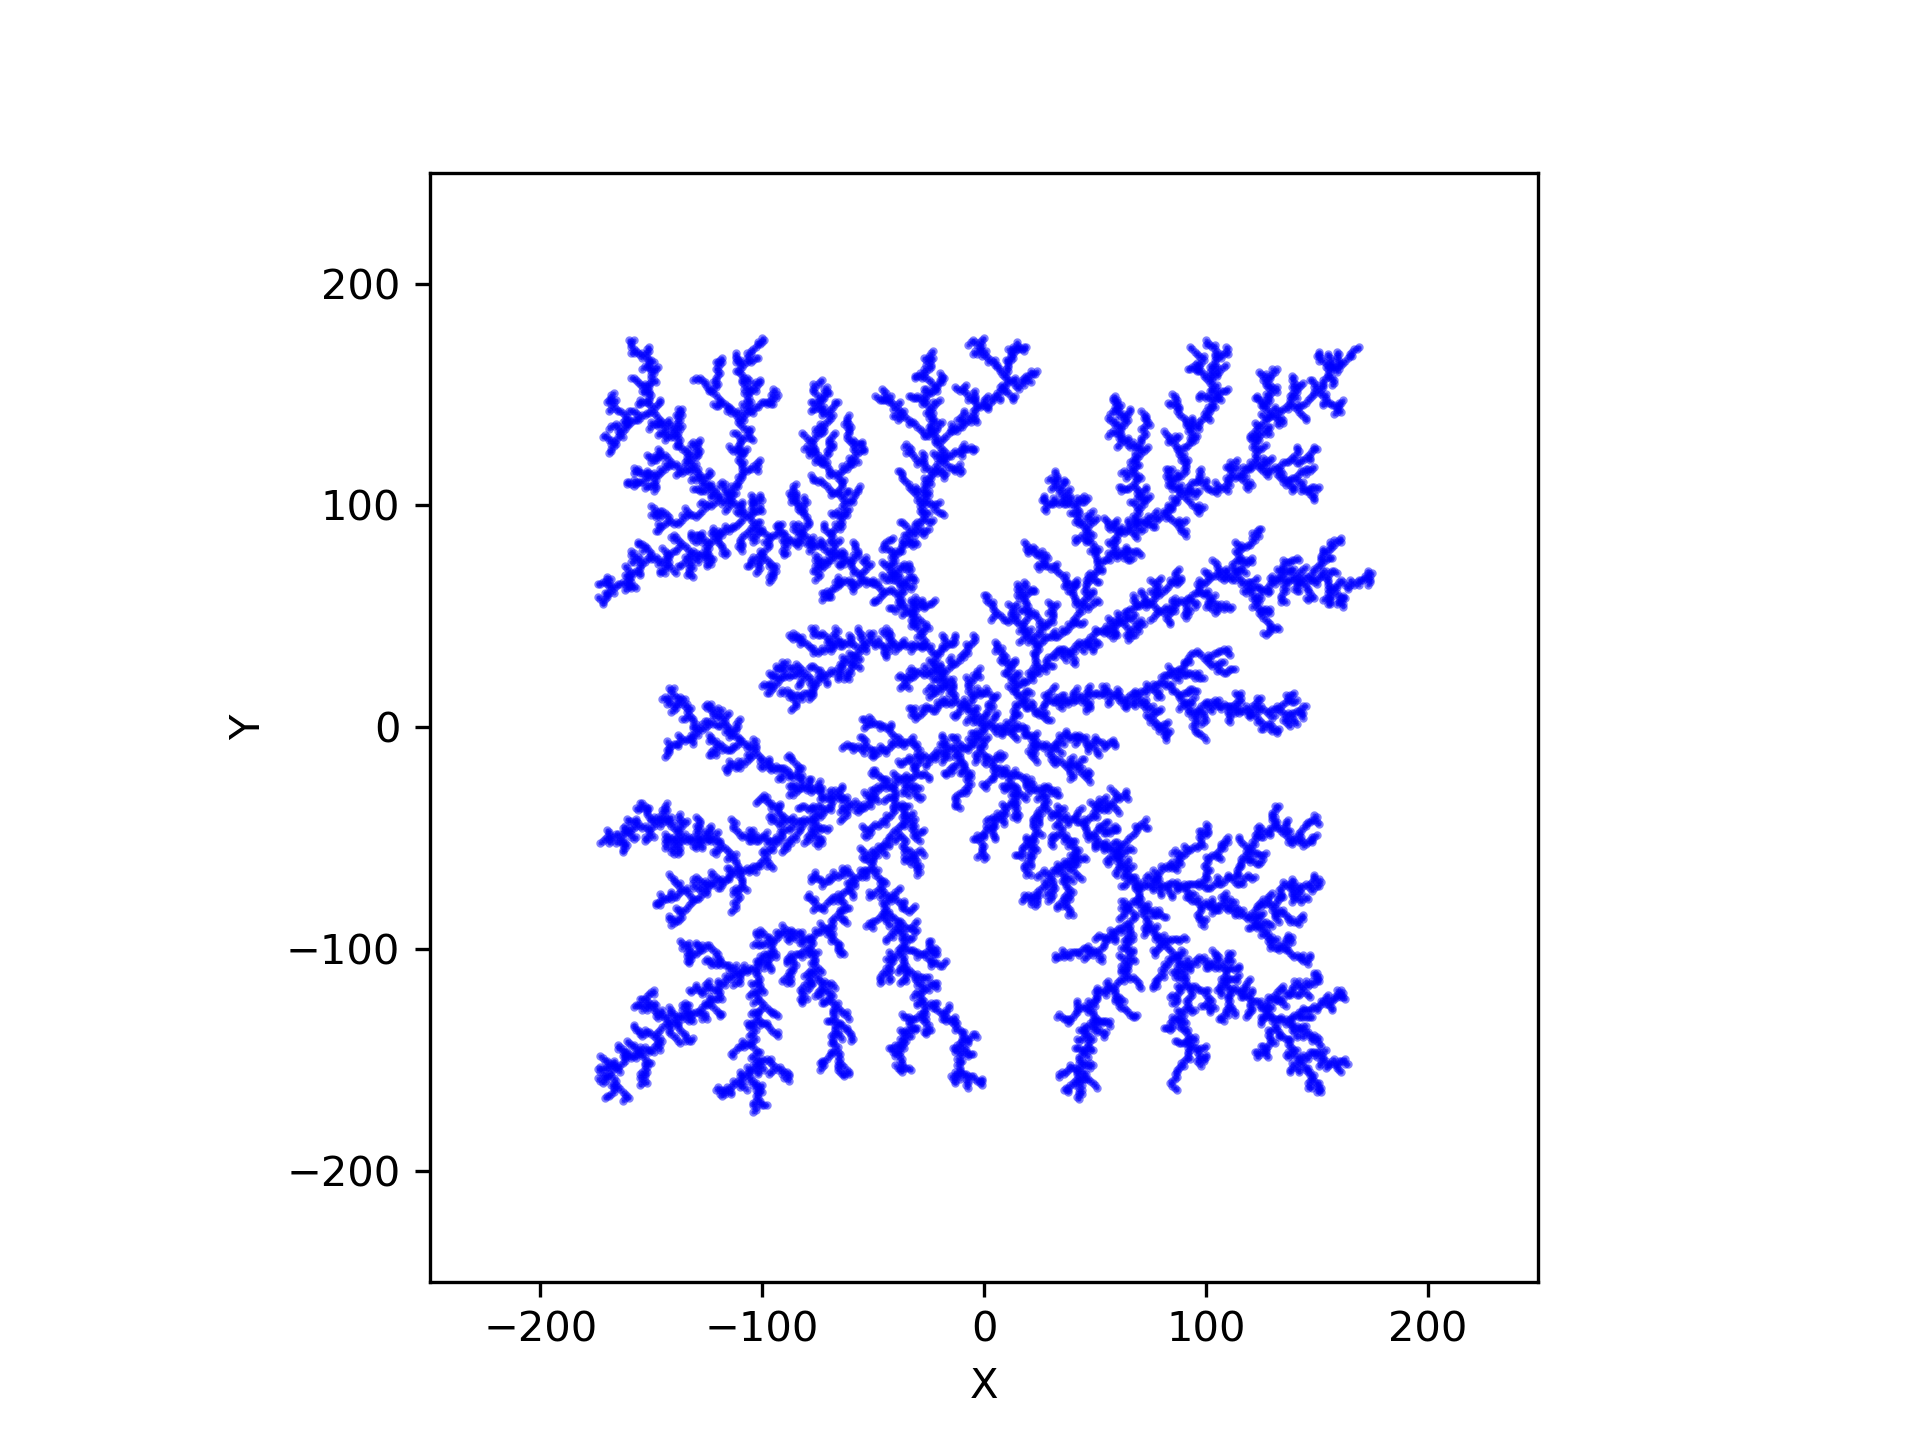
\includegraphics[bb= 0 0 460.8 345.6, width = 10cm]{500-104-1.png}      
\caption{正方形边界$10^{4}$个粒子的可视化模拟结果}      
\end{figure}

\newpage
不均匀性的出现也十分好理,因为在正方形边缘上均匀分布的随机点在角度上的分布显然不均匀,4个角处的分布更加密集。


\section{心得与体会}
通过此次作业,对DLA模型有了更加深刻的认识,且对计算分形维数的方法更加熟练。更加深刻的体会到计算模拟程序中模拟更加准确与耗费资源时间之间的矛盾。


\newpage
\section{附录}

\begin{appendices}


\section{DLA模拟C语言源程序}
\begin{lstlisting}[language = C]
#include <stdio.h>
#include <stdlib.h>
#include <math.h>
#include <string.h>
#define a 16807
#define b 0
#define m 2147483647
#define r (m%a)
#define q (m/a)
#define Pi 3.1415926
#define ROUND(x) ((x)>=0?(int)((x)+0.5):(int)((x)-0.5))
#define GETMATELEM(base,i,j,imax) ((*(base + (i) * (imax) + (j)))) //取二维数组元素
#define LEN 1500  //DLA位置数组的 X or Y 轴长度的一半


//利用/dev/random 产生"真"随机数
int my_realrandom(int ran[],int n){
    FILE *fp1 = fopen("/dev/random","r");
    for(int i=0;i<n;i++){
        fread(&ran[i], 1, 4, fp1);
    }
    fclose(fp1);
    return 0;
}



int my_filewriter_int(char str[],int num[],int n){
    FILE * fp;
    fp = fopen(str,"w+");
    
    for(int i=0;i<n;i++)
    {
        if (i == (n-1)){
            fprintf(fp,"%d",num[i]);
            break;
        }
        fprintf(fp,"%d,",num[i]);
        
    }
    fclose(fp);
    return 0;
}


int my_filereader_int(char str[],int num[],int n){
    FILE * fp;
    fp = fopen(str,"r");

    for(int i=0;i<n-1;i++)
    {
        fscanf(fp,"%d,",&num[i]);

    }
    fscanf(fp,"%d",&num[n-1]);    //最后一个数据后不加 ","
    fclose(fp);
    return 0;
}



// Schrage 方法产生随机数
int my_schrage(double ran[],int seed,int n){
    for (int i = 0; i < n - 1; i++) {
        if (seed >= 0) {
            ran[i] = seed / (double) m;
        } else {
            ran[i] = (seed + m) / (double) m;
        }
        if(seed == m-1){
            if(a >=  b){    //由于Schrage方法只对z in (0,m-1)成立,故这里要讨论z == m-1的情况
                seed = m + (b-a) % m;
            }
            else   seed =  (b-a) % m;

        }
        else seed = ((a * (seed % q) - r * (seed /  q)) + b % m ) % m;  //递推式
    }
    if (seed >= 0) {
        ran[n-1] = seed / (double) m;
    } else {
        ran[n-1] = (seed + m) / (double) m;
    }
    return 0;
}






// Schrage 方法迭代器
int my_schrage_iter(int seed){
    if(seed == m-1){
        if(a >=  b){    //由于Schrage方法只对z in (0,m-1)成立,故这里要讨论z == m-1的情况
            seed = m + (b-a) % m;
        }
        else   seed =  (b-a) % m;

    }
    else seed = ((a * (seed % q) - r * (seed /  q)) + b % m ) % m;  //递推式
    
    return seed;
}


int randomparticle(double ran,int min,int *i,int *j){   //产生随机粒子的初始位置
    double theta = 2*Pi*ran;  //为了使初始位置更加均匀,我们取圆形边界,产生均匀分布的随机角度值
    double x = min*cos(theta);  //以min为半径,计算此初始位置相对于原点的x,y值
    double xf = x-floor(x);  //x的小数部分
    double y = min*sin(theta);
    double yf = y-floor(y);  //y的小数部分
    *i = (int)( LEN + floor(x) + floor(2*xf) ); //结束后,i,j变为初始位置的矩阵坐标
    *j = (int)( LEN + floor(y) + floor(2*yf) );
    
    
    /*   //以下为正方形边界
    int n = (int)floor(8*min*ran); //粒子位于边缘处的哪个位置
    //printf("n= %d\n",n);
    
    if (n < 2*min+1){  //一下过程均为找到此位置的行号和列好
        *i = LEN-min;
        *j = LEN-min+n;
        return 0;
    }
    else n -= 2*min;
    if (n < 2*min+1){
        *i = LEN-min+n;
        *j = LEN+min;
        return 0;
    }
    else n -= 2*min;
    if (n < 2*min+1){
        *i = LEN+min;
        *j = LEN+min-n;
        return 0;
    }
    else n -= 2*min;
    *i = LEN+min-n;
    *j = LEN-min;
    */
    return 0;
}


int particleRW(int *o,int *p,int max,int *position,int seed){ //产生的随机粒子随机行走器 //o,p为初始粒子的位置,max为判定粒子逃逸的范围,position为总位置坐标数组
    int i = *o;
    int j = *p;
    double ran;
    int flag = 0;
    for(int k = -1;k<2;k++){  //查看粒子周围是否有团簇粒子,有的话flag != 0
        for(int l = -1;l<2;l++){
            flag += GETMATELEM(position, (i-k), (j-l), (2*LEN+1));
        }
    }
    while (flag == 0 && sqrt( pow(i-LEN,2)+pow(j-LEN,2) ) < max ){  //粒子周围没有团簇粒子且在逃逸区域以内,则继续随机行走
        if (seed >= 0) {
            ran = seed / (double) m;
        }
        else {
            ran = (seed + m) / (double) m;
        }
        if(ran<0.25) j +=1 ;   //4个方向随机行走
        else if(ran<0.5 && ran >= 0.25) j -= 1;
        else if(ran<0.75 && ran>=0.5 ) i += 1;
        else i -= 1;
        seed = my_schrage_iter(seed);
        for(int k = -1;k<2;k++){  //查看粒子周围是否有团簇粒子,有的话flag != 0
            for(int l = -1;l<2;l++){
                flag += GETMATELEM(position, (i-k), (j-l), (2*LEN+1));
            }
        }
    }
    if(flag == 0) return 1;  //此时粒子逃逸,需要重新模拟
    *o = i;
    *p = j;
    return 0;   //结束后i,j变为此粒子最终的位置
}

int boxcount(int* position,int *count,int Len,int maxr){  //盒计数法统计N,Len为位置二维数组的半径,maxr,为统计范围的半径
    int flag = 0;
    int n = 0;  //区域内是否有粒子的累加器
    int len;
    if( (2*Len) < 2*maxr ){
        printf("LEN is too short to count");
        return 1;
    }
    for(int i = 1; i < 2*maxr + 1; i = i*2){
        len = 2*maxr/i;
        for(int k = 0 ;k < i ; k++){  //方格计数
            for(int l = 0 ;l < i ; l++){
                n = 0;
                for(int o = Len - maxr + len*k; o < Len - maxr +len*(k+1); o++){
                    for(int p = Len - maxr + len*l; p < Len - maxr +len*(l+1); p++ ){
                        n += GETMATELEM(position, o, p, (2*Len+1));
                    }
                }

                if (n != 0) count[flag] += 1;
            }
        }
        flag++;
    }
    return 0;
}


int sandboxcount(int*position, int*count,int rmax,int Len){ //sandbox法统计N,rmax为统计区域的半径最大值,Len为位置二维矩阵的半径
    int radius = 5;  //起始统计范围半径为5
    int flag = 0;
    int n = 0;
    for(;radius < rmax + 1;radius += 5){  //统计范围半径依次增加5
        n = 0;
        for(int i = Len - radius; i < Len + radius; i++){
            for(int j = Len - radius; j < Len + radius; j++){
                n += GETMATELEM(position, i, j, (2*Len+1));
            }
        }
        count[flag] = n;
        flag++;
    }
    return 0;
}


    
int main(int argc, const char * argv[]) {
   
    
    int N = 50000;  //粒子总数
    int min,max;  //分别对应产生粒子的区域和判断粒子逃逸的范围
    min = 5;
    max = 205 ;
    int i,j;
    int *position = malloc(sizeof(int)*(2*LEN+1)*(2*LEN+1));  //存放位置坐标的数组
    
    for(int i =0;i<(2*LEN+1)*(2*LEN+1);i++){   //位置坐标初始化
        position[i] = 0;
    }
 
    GETMATELEM(position, (LEN), (LEN), (2*LEN+1)) = 1; //设定原点(0,0)处初始有一粒子
    
    int *seed = malloc(sizeof(int)*N);  //随机数种子
    my_realrandom(seed, N);
    double *ran = malloc(sizeof(double)*N);  //每次粒子的初始位置
    my_schrage(ran, seed[0], N);
    int flag = 0;
    for(int k =0;k<N;k++){
        flag = 0;
        randomparticle(ran[k], min,&i, &j);
        flag = particleRW(&i, &j, max, position, seed[k]);
        if(flag == 1){
            while (flag == 1) {
                flag = 0;
                my_realrandom(&seed[k], 1);
                flag = particleRW(&i, &j, max, position, seed[k]);
            }
        }
        GETMATELEM(position, (i), (j), (2*LEN+1)) = 1;
        if(abs(i-LEN) > min-5) min = 5 + abs(i-LEN);
        if(abs(j-LEN) > min-5) min = 5 + abs(j-LEN);
        max = min + 200 ;
    }
    my_filewriter_int("p.dat", position, (2*LEN+1)*(2*LEN+1));    
        
    return 0;
}

\end{lstlisting}



\newpage

\section{分形维数统计C语言程序源码}
\begin{lstlisting}[language = C]
#include <stdio.h>
#include <stdlib.h>
#include <math.h>

int my_filereader_int(char str[],int num[],int n){
    FILE * fp;
    fp = fopen(str,"r");

    for(int i=0;i<n-1;i++)
    {
        fscanf(fp,"%d,",&num[i]);

    }
    fscanf(fp,"%d",&num[n-1]);    //最后一个数据后不加 ","
    fclose(fp);
    return 0;
}

int boxcount(int* position,int *count,int Len,int maxr){  //盒计数法统计N,Len为位置二维数组的半径,maxr,为统计范围的半径
    int flag = 0;
    int n = 0;  //区域内是否有粒子的累加器
    int len;
    if( (2*Len) < 2*maxr ){
        printf("LEN is too short to count");
        return 1;
    }
    for(int i = 1; i < 2*maxr + 1; i = i*2){
        len = 2*maxr/i;
        for(int k = 0 ;k < i ; k++){  //方格计数
            for(int l = 0 ;l < i ; l++){
                n = 0;
                for(int o = Len - maxr + len*k; o < Len - maxr +len*(k+1); o++){
                    for(int p = Len - maxr + len*l; p < Len - maxr +len*(l+1); p++ ){
                        n += GETMATELEM(position, o, p, (2*Len+1));
                    }
                }

                if (n != 0) count[flag] += 1;
            }
        }
        flag++;
    }
    return 0;
}


int sandboxcount(int*position, int*count,int rmax,int Len){ //sandbox法统计N,rmax为统计区域的半径最大值,Len为位置二维矩阵的半径
    int radius = 5;  //起始统计范围半径为5
    int flag = 0;
    int n = 0;
    for(;radius < rmax + 1;radius += 5){  //统计范围半径依次增加5
        n = 0;
        for(int i = Len - radius; i < Len + radius; i++){
            for(int j = Len - radius; j < Len + radius; j++){
                n += GETMATELEM(position, i, j, (2*Len+1));
            }
        }
        count[flag] = n;
        flag++;
    }
    return 0;
}



int main(int argc, const char * argv[]) {
 	int len = 512;
    int Len = 1500;
    int *position = malloc(sizeof(int)*(2*Len+1)*(2*Len+1));
    int *count1 = malloc(sizeof(int)*11);  //盒计数法统计N存放数组
    int *count2 = malloc(sizeof(int)*60);  //Sandbox法统计N存放数组
    
    for (int i = 0;i<11;i++){  //数组初始化
        count1[i] = 0;
    }
    
    for (int i = 0;i<60;i++){    //数组初始化
           count2[i] = 0;
       }
    
    my_filereader_int("p-1500-5*104-5-2*min.dat", position, (2*Len+1)*(2*Len+1)); //读取之前生成的位置矩阵

    boxcount(position, count1, Len, len);
    sandboxcount(position, count2, 300,Len);
    
    my_filewriter_int("box.txt", count1, 11);
    my_filewriter_int("sandbox.txt", count2, 60);
          
    return 0;
}	
\end{lstlisting}





\newpage

\section{可视化绘图及数据处理Python程序源码}

\begin{lstlisting}[language = python]
iimport matplotlib.pyplot as plt
import numpy as np
import math

plt.rcParams['savefig.dpi'] = 300 #图片像素
plt.rcParams['figure.dpi'] = 300 #分辨率
# 默认的像素:[6.0,4.0],分辨率为100,图片尺寸为 600&400
fig1 = plt.figure()
fig2 = plt.figure()
fig3 = plt.figure()
max = 500  #团簇位置信息二维矩阵半径
ax1 = fig1.add_subplot(111)
ax2 = fig2.add_subplot(111)
ax3 = fig3.add_subplot(111)



X = []
Y = []
y = []
box = []
sandbox = []
xbox = []
xsandbox = []

xtbox = []
xtsandbox = []


with open('problem 13/p-500-104-1.dat', 'r') as f:
    while True:
        lines = f.readline() # 整行读取数据
        if not lines:
            break
        y = [float(i) for i in lines.split(',')]  # 将整行数据分割处理
    y = np.array(y) # 将数据从list类型转换为array类型。


with open('problem 13/box-5-3*min.txt', 'r') as f:
    while True:
        lines = f.readline() # 整行读取数据
        if not lines:
            break
        box = [float(i) for i in lines.split(',')]  # 将整行数据分割处理
    box = np.array(box) # 将数据从list类型转换为array类型。


with open('problem 13/sandbox-5-3*min.txt', 'r') as f:
    while True:
        lines = f.readline() # 整行读取数据
        if not lines:
            break
        sandbox = [float(i) for i in lines.split(',')]  # 将整行数据分割处理
    sandbox = np.array(sandbox) # 将数据从list类型转换为array类型。

for i in range(pow(2*max+1, 2)):
    if y[i] != 0:
        X.append(i % (2*max+1)-max)
        Y.append(max - i/(2*max+1))

box = np.delete(box, 10)   #是否排除盒计数法最后一个数据点
print(box)

box = np.log(box)     # 盒计数法横轴数据点生成
xbox = np.ones(len(box))
for i in range(len(box)):
    xbox[i] = math.log(pow(2, i))

sandbox = np.log(sandbox)  # Sandbox法横轴数据点生成
xsandbox = np.ones(60)
for i in range(60):
    xsandbox[i] = math.log(5 + i*5)


[ab, bb] = np.polyfit(xbox, box, 1)   # 两计算分形维数方法的线性拟合
[asb, bsb] = np.polyfit(xsandbox, sandbox, 1)
print([ab, bb])
print([asb, bsb])


ax1.scatter(X, Y, c='b', label='', s= 1, alpha=0.5, marker='o')  # DLA模拟结果散点图
ax1.set_xlabel('X')
ax1.set_ylabel('Y')
ax1.set_xlim(-max/2, max/2)
ax1.set_ylim(-max/2, max/2)
ax1.set_aspect('equal')
fig1.savefig("1.png")


ax2.scatter(xbox, box, c='b', label='Computing data', s= 1, alpha=0.5, marker='o')  # 盒计数法对数图
ax2.plot(xbox, ab*xbox+bb, lw=0.5, color='r', label='Linear Fitting Curve')
ax2.set_xlabel(r'$ln(1/ \epsilon)$')
ax2.set_ylabel(r'$lnN$')
ax2.legend(loc=2)
ax2.text(0, 9, r"$lnN=$"+str(ab)+r'$\times ln(1/ \epsilon)+$'+str(bb), fontsize=8, color="black")
fig2.savefig("2.png")

ax3.scatter(xsandbox, sandbox, c='b', label='Computing data', s= 1, alpha=0.5, marker='o')  # sandbox对数图
ax3.plot(xsandbox, asb*xsandbox+bsb, lw=0.5, color='r', label='Linear Fitting Curve')
ax3.set_xlabel(r'$lnr$')
ax3.set_ylabel(r'$lnN$')
ax3.text(1.5, 9, r"$lnN=$"+str(asb)+r'$\times ln(r)+$'+str(bsb), fontsize=8, color="black")
ax3.legend(loc=2)
fig3.savefig("3.png")

\end{lstlisting}


\end{appendices}




\end{document}
